\chapter{Results and Analysis}
\label{chapterlabel5}

\section{Performance Comparison between Dynamic Author-Topic and LDA Models}\label{sec:ldadat}

The parameters of LDA  model is set as $\alpha = 0.01$, $\beta = 0.01$, with no authors.
While, for Dynamic Author-topic model the $\alpha$  is initialized as 0.1, and $\beta$ is initialized as 0.01. For DAT model we set $\text{Author Number} = 9$ with other parameters the same as LDA. 

\subsection{Perplexity}
The perplexity comparison between LDA and DAT model is shown in Figure ~\ref{fig:lda_dat_perplexity}, to answer \textbf{RQ6}. A lower perplexity score indicates a better generalization performance of the model. Figure ~\ref{fig:lda_dat_perplexity} shows that our DAT model performs poorer than LDA early on but with more prior information are introduced we see the cross-over point where DAT model adapts better to our news corpus. And with the increasing number of topic numbers, we observe that both model performs better while DAT is more adaptive which answers \textbf{RQ5}. The inferior performance of DAT with low number of topic number is that our author number is fixed as 9 which restrict the flexibility of topic assignment to the news, and author assignments become randomly in this case.

\begin{figure}[h]
\centering
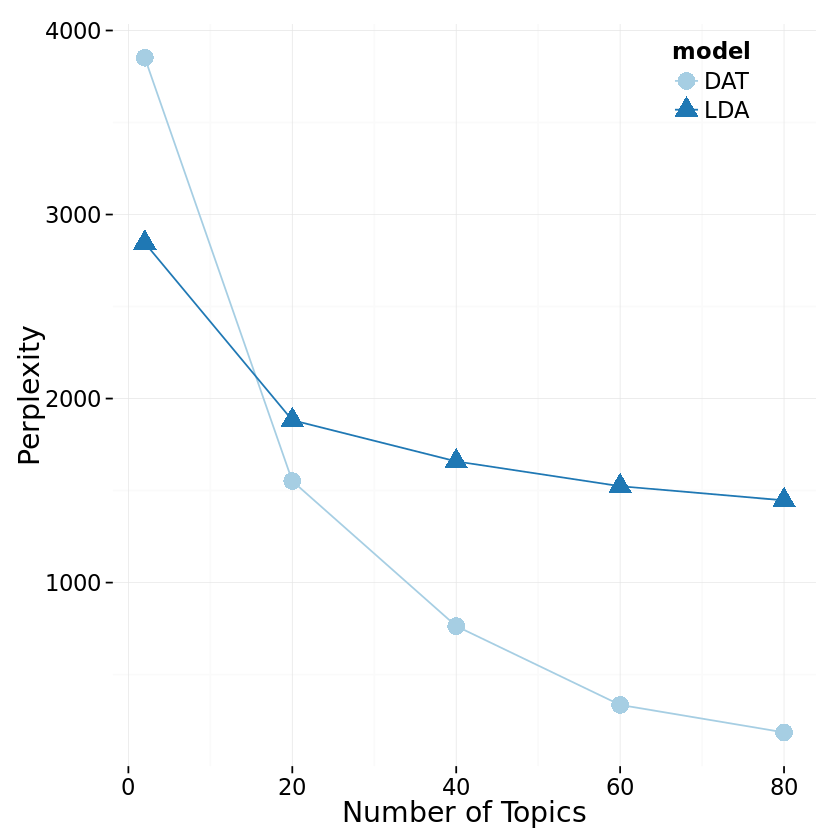
\includegraphics[width=1\textwidth]{figures/lda_dat_perplexity.png}
\caption{Mean perplexity of DAT and LDA with varying numbers of latent topics.}
\label{fig:lda_dat_perplexity}
\end{figure}

\subsection{Topic Distribution}
Here we try to evaluate the classification performance of the two model in order to answer \textbf{RQ1,3, 4}. The topic number $K$ is set as 20 here for expriment purpose. Topic- category distribution for LDA model is shown in Figure ~\ref{fig:lda_with_weights} with the instruction in Section ~\ref{sec:topicassignment} to evaluate the news segmentation, the facet wrap plot shows for each topic (1 to 20) how many articles are tagged with 1 of the 8 categories (the articles falling in category \textit{politics} are all also with category tag of \textit{UK} or \textit{world}, so articles with tag \textit{politics} are ignored here  ). From Figure ~\ref{fig:lda_with_weights} we can observe that using LDA model the topic segmentation is prominent since for in most (18 our of 20) of the topics there is only one category dominating the tohers in terms of article number. For example, after training with LDA model, in total about 100 articles are assigned to \textit{Topic 4} which is on the upper right corner in Figure ~\ref{fig:lda_with_weights}, where 62 articles are co-tagged with category \textit{entertainment} as predefined. This co-occurrence indicates that \textit{Topic 4} can be manually interpreted as \textit{entertainment}. This can be double-checked with viewing the most relevant words for each topic where appropriate shown in Table ~\ref{table:ldatopicdistribution}
\begin{figure}[h]
\centering
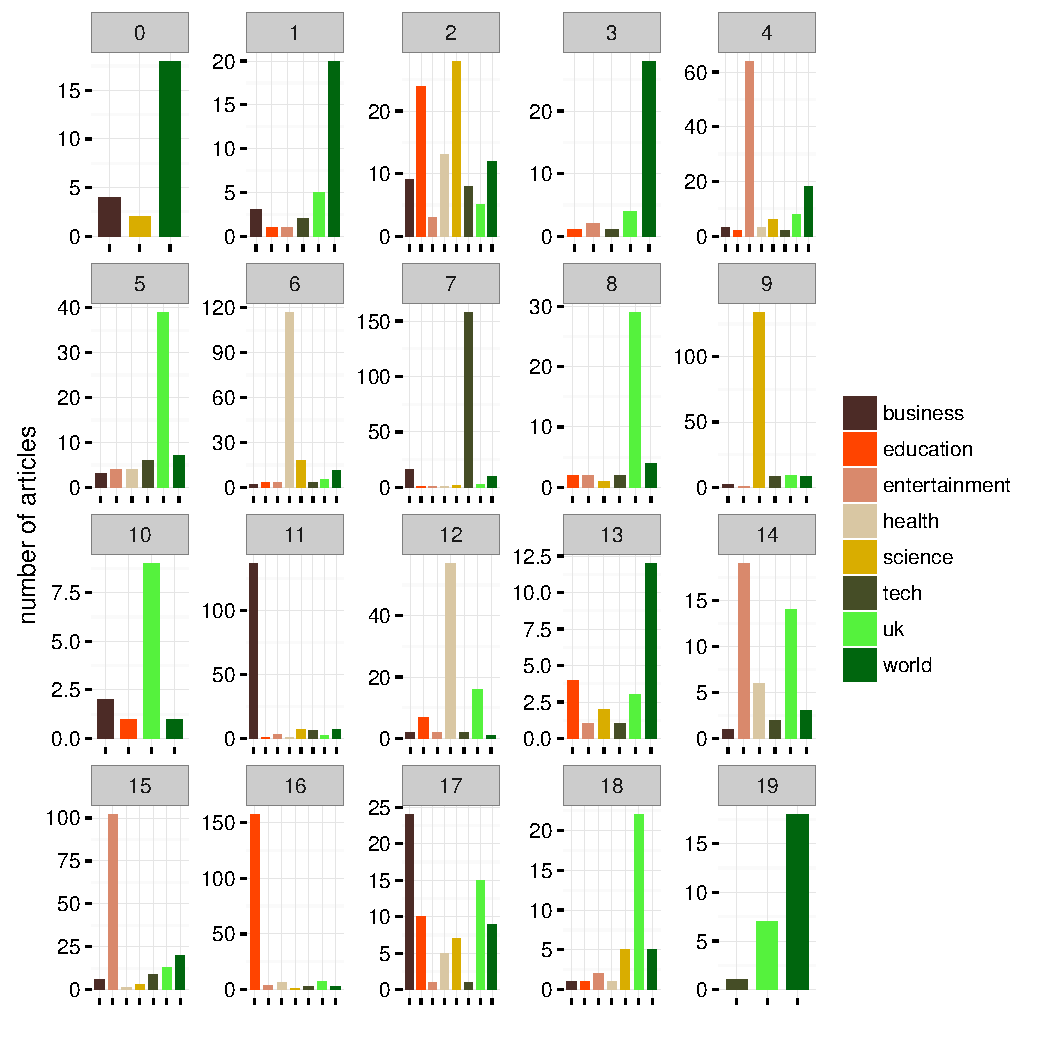
\includegraphics[width=1\textwidth]{figures/lda_with_weights.pdf}
\caption{Topic-Categoy distribution of LDA model.}
\label{fig:lda_with_weights}
\end{figure}

\begin{table}[h!]
\centering
\begin{tabular}{|c c|} 
\hline
\multicolumn{2}{|c|}{\textbf{Topic 4 : Entertainment}} \\
\hline
 \textbf{WORD} & \textbf{PROB}.  \\ [0.3ex] 
 \hline
 	like  &   0.006608  \\ 
	go   &  0.004549  \\ 
	get   &  0.004535  \\ 
	bbc   &  0.004427  \\ 
	first   &  0.004388  \\ 
	show   &  0.004210  \\ 
	work   &  0.004058  \\ 
	music   &  0.003949  \\ 
	world   &  0.003945  \\ 
	day   &  0.003721  \\ 
	think  &   0.003566  \\ 
	story  &   0.003566  \\ 
	want   &  0.003407  \\ 
	many   &  0.003295  \\ 
	make   &  0.003272  \\ 
	play   &  0.003266  \\ 
	see   &  0.003152  \\ 
	look   &  0.003120  \\ 
	live   &  0.003073  \\ 
	thing  &   0.003016 \\ [1ex] 
 \hline
  
\end{tabular}
 \hfill
 \begin{tabular}{|c c|} 
\hline
\multicolumn{2}{|c|}{\textbf{Topic 6 : Health}} \\
\hline
 \textbf{WORD} & \textbf{PROB}.  \\ [0.3ex] 
 \hline
 health &   0.014923 \\
	hospital  &     0.010606 \\
	patient &      0.009591 \\
	cancer  &     0.007800 \\
	baby  &     0.006598 \\
	drug   &    0.006186 \\
	dry   &    0.006108 \\
	case   &    0.005651 \\
	medic  &     0.005632 \\
	treatment  &     0.005485 \\
	disease   &    0.005480 \\
	research   &    0.005440 \\
	women   &    0.004857 \\
	doctor  &     0.004646 \\
	risk   &    0.004567 \\
	death  &     0.004528 \\
	nhs  &     0.004405 \\
	zika  &     0.004332 \\
	cause   &    0.004243 \\
	virus   &    0.004239 \\ [1ex] 
 \hline
  
\end{tabular}
\hfill
\begin{tabular}{|c c|} 
\hline
\multicolumn{2}{|c|}{\textbf{Topic 7 : Tech}} \\
\hline
 \textbf{WORD} & \textbf{PROB}.  \\ [0.3ex] 
 \hline
 company &  0.009285 \\
	data  &   0.006523 \\
	firm   &  0.005587 \\
	could   &  0.005347 \\
	service  &   0.005159 \\
	inform  &   0.004911 \\
	bbc   &  0.004890 \\
	make   &  0.004840 \\
	user   &  0.004722 \\
	report  &   0.004550 \\
	phone  &   0.004487 \\
	online   &  0.004432 \\
	technology  &   0.004424 \\
	work   &  0.004378 \\
	secure  &   0.004328 \\
	system  &   0.004218 \\
	custom  &   0.003841 \\
	call  &   0.003841 \\
	compute  &   0.003841 \\
	facebook   &  0.003761 \\ [1ex] 
 \hline
 
 \end{tabular} 
\\[1cm]
 \begin{tabular}{|c c|} 
\hline
\multicolumn{2}{|c|}{\textbf{Topic 9 : Science}} \\
\hline
 \textbf{WORD} & \textbf{PROB}.  \\ [0.3ex] 
 \hline
 site  & 0.006374  \\ 
	project  &   0.005936  \\ 
	plan   &  0.005232  \\ 
	work   &  0.004813  \\ 
	build   &  0.004781  \\ 
	develop  &   0.004430  \\ 
	could &    0.004268  \\ 
	area  &   0.004226  \\ 
	space  &   0.004213  \\ 
	plant  &   0.003632  \\ 
	land   &  0.003531  \\ 
	first  &   0.003512  \\ 
	water   &  0.003401  \\ 
	uk   &  0.003226  \\ 
	part  &   0.003119  \\ 
	found  &   0.003074  \\ 
	animal  &  0.002915  \\ 
	energy  &   0.002863  \\ 
	world   &  0.002811  \\ 
	design   &  0.002781 \\ [1ex] 
 \hline
  
 \end{tabular}
 \hfill
 \begin{tabular}{|c c|} 
\hline
\multicolumn{2}{|c|}{\textbf{Topic 11 : Business}} \\
\hline
 \textbf{WORD} & \textbf{PROB}.  \\ [0.3ex] 
 \hline
 company  & 0.012396 \\
	price  &  0.011260\\
	market &   0.011054\\
	bank  &  0.009842\\
	business &   0.008478\\
	oil  &  0.007454\\
	share &   0.006968\\
	sale &   0.006634\\
	china &   0.006157\\
	firm  &  0.006066\\
	growth &   0.005923\\
	rate &   0.005726\\
	uk  &  0.005698\\
	economy &   0.005410\\
	month  &  0.005285\\
	report &   0.004745\\
	invest &   0.004720\\
	product &   0.004681\\
	trade &   0.004654 \\
	fall  & 0.004614 \\[1ex] 
 \hline
  
 \end{tabular}
 \hfill
 \begin{tabular}{|c c|} 
\hline
\multicolumn{2}{|c|}{\textbf{Topic 16 : Education}} \\
\hline
 \textbf{WORD} & \textbf{PROB}.  \\ [0.3ex] 
 \hline
 school  & 0.029979 \\
	children   &  0.012832 \\
	council    & 0.008763 \\
	educate    & 0.008570 \\
	teacher   &  0.008009 \\
	report   &  0.007690 \\
	pupil   &  0.007396 \\
	work   &  0.005670 \\
	parent   &  0.005087 \\
	need   &  0.005065 \\
	govern    & 0.004812 \\
	staff   &  0.004794 \\
	service  &  0.004671 \\
	support   &  0.004404 \\
	concern   &  0.004159 \\
	issue    & 0.003980 \\
	plan    & 0.003943 \\
	child   &  0.003765 \\
	primary   &  0.003743 \\
	improve   & 0.003702 \\ [1ex] 
 \hline
  
 \end{tabular}
\caption{LDA Topic-Word distribution}
\label{table:ldatopicdistribution}
\end{table}

In Table ~\ref{table:ldatopicdistribution} we have selected 6 topics to show its top 20 words with highest probabilities conditioned on the topics. The title of the topic is our manual interpretation based on Figure ~\ref{fig:lda_with_weights}. It is easily to see that for each table the words are definitely relevant to the topic itself. For example, for \textit{Topic 6, health} we can see the words like \textit{hostipital, petient, cancer, drug, treatment, zika, NHS, virus}, etc. and for \textit{Topic 16, education}, we see words like \textit{school, children, teacher, staff, primary, improve}, etc, which are all type of words for \textit{education}. 

However, although the topics segmentation is clear for LDA model, we see two drawbacks with the model.
\begin{itemize}
    \item Firstly, we cannot see the trends of the news, namely how the topics rise and fall for a certain news event. Therefore we see the words for each topic is just general words spreading through the time, for example, if we look at the words for \textit{Topic 7, tech}, it is obviously that all the words are describing technology itself however it is hardly to speculate what kind of news is happening specifically.
    \item Secondly, LDA model will confound the topics between different news event. For example, for \textit{Topic 6, health}, the words \textit{drug, treatment, hospital} are related to the events that in May the NHS will not fund anti-HIV Prep drug plan \footnote{http://www.bbc.co.uk/news/health-36421124}, while \textit{zika} and \textit{virus} are extracted from the news events of the devastating epidemic Zika virus in Africa \footnote{http://www.bbc.co.uk/news/health-36379455}. It is not clear what news events are captured by LDA model exactly. 
\end{itemize}

Then for DAT model, we are now running the experiment based on short-term dependency with time-period as a week. In total there are 22 weeks spreading the whole corpus, we have selected 4 of them for investigation.
Topic category distribution for DAT model is shown in Figure ~\ref{subfig:11dattopiccategory} (From Jan 1 to Jan 7), Figure ~\ref{subfig:212dattopiccategory} (From Feb 12 to Feb 19), Figure ~\ref{subfig:34dattopiccategory} (From Jan Mar 4 to Mar 11), and Figure ~\ref{subfig:520dattopiccategory} (From May 20 to May 27).

Using the same way as for exploring LDA model as above, for the four different weeks we firstly find the prominence category for each topic which will be the topic's representative, and secondly we check the most relevant words associated with each topic to see whether they are valid to discover news events.


\begin{figure*}[!t]
  \centering
    \subfigure[2016.01.01 to 2016.01.07]{
    \label{subfig:11dattopiccategory} 
    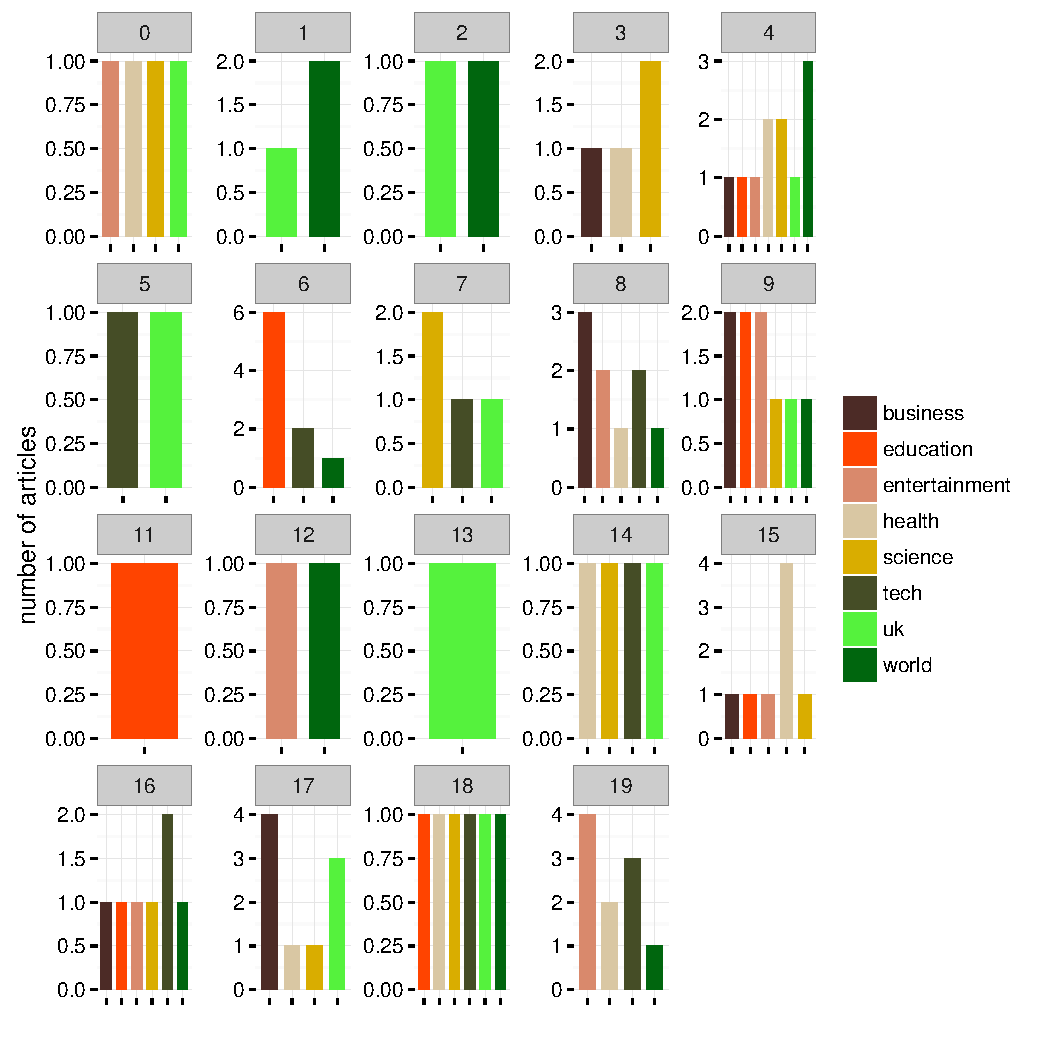
\includegraphics[width=.48\columnwidth]{figures/11datcatogery.pdf}}
    \subfigure[2016.02.12 to 2016.02.19]{
    \label{subfig:212dattopiccategory} 
    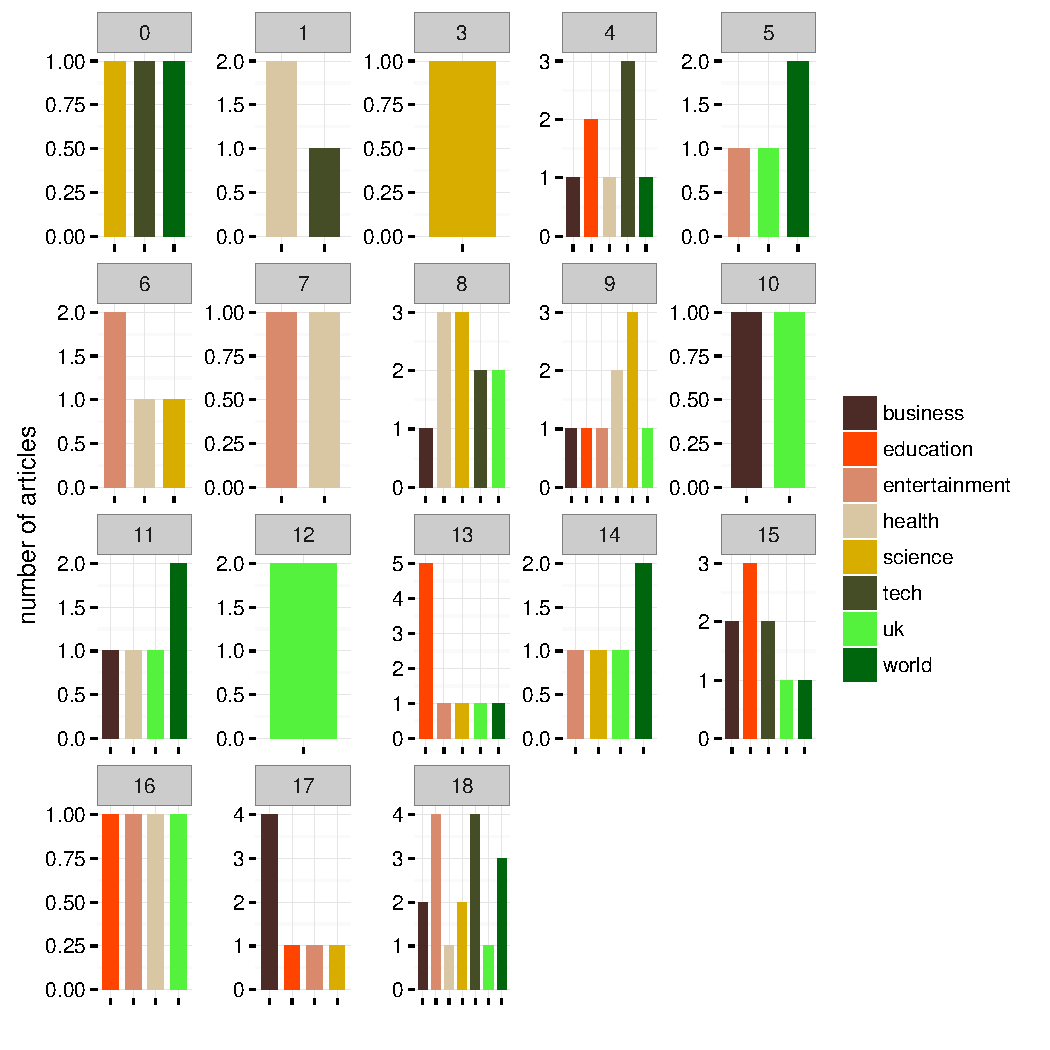
\includegraphics[width=.48\columnwidth]{figures/212datcatogery.pdf}}
    \vspace*{-.9\baselineskip}
    \subfigure[2016.03.04 to 2016.03.11]{
    \label{subfig:34dattopiccategory} 
    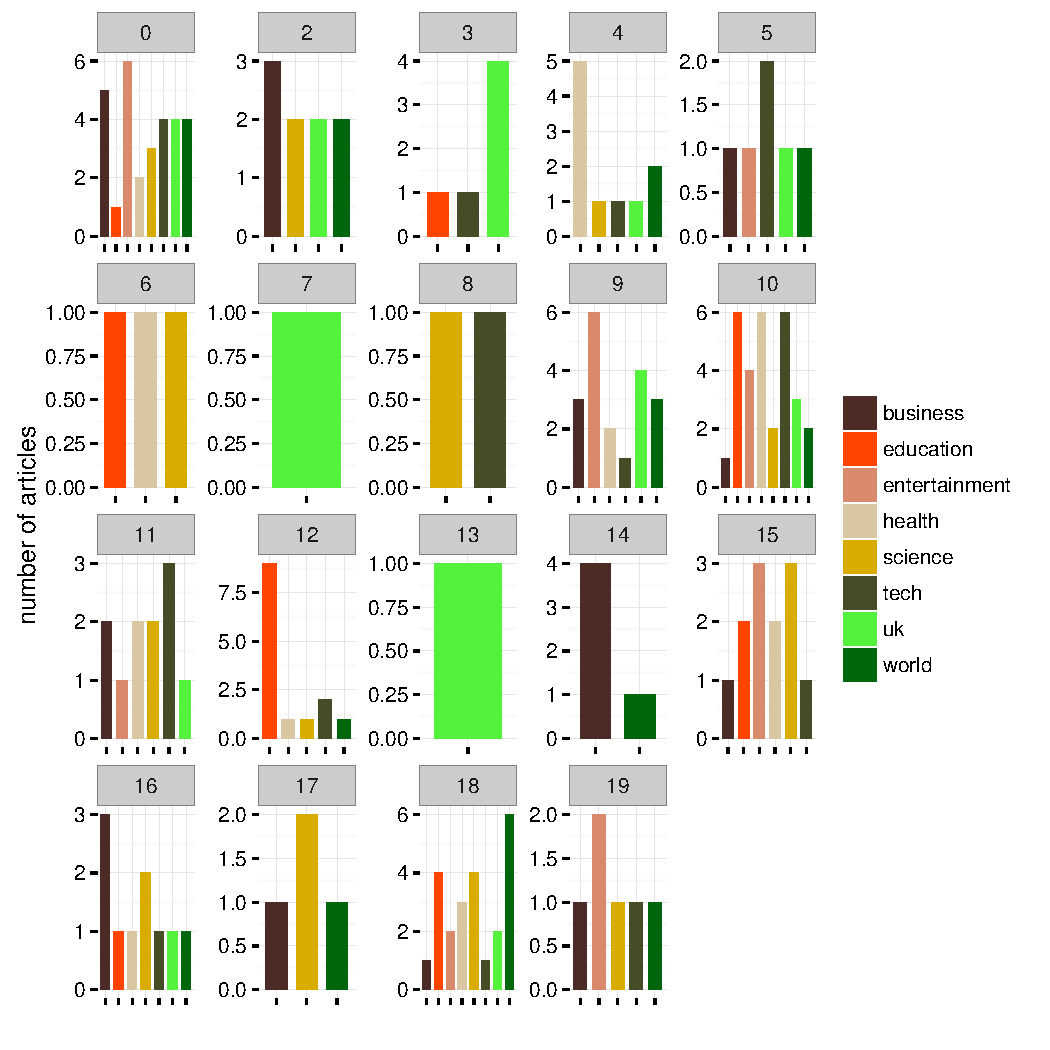
\includegraphics[width=.48\columnwidth]{figures/34datcatogery.pdf}}
    \subfigure[2016.05.20 to 2016.05.27]{
    \label{subfig:520dattopiccategory} 
    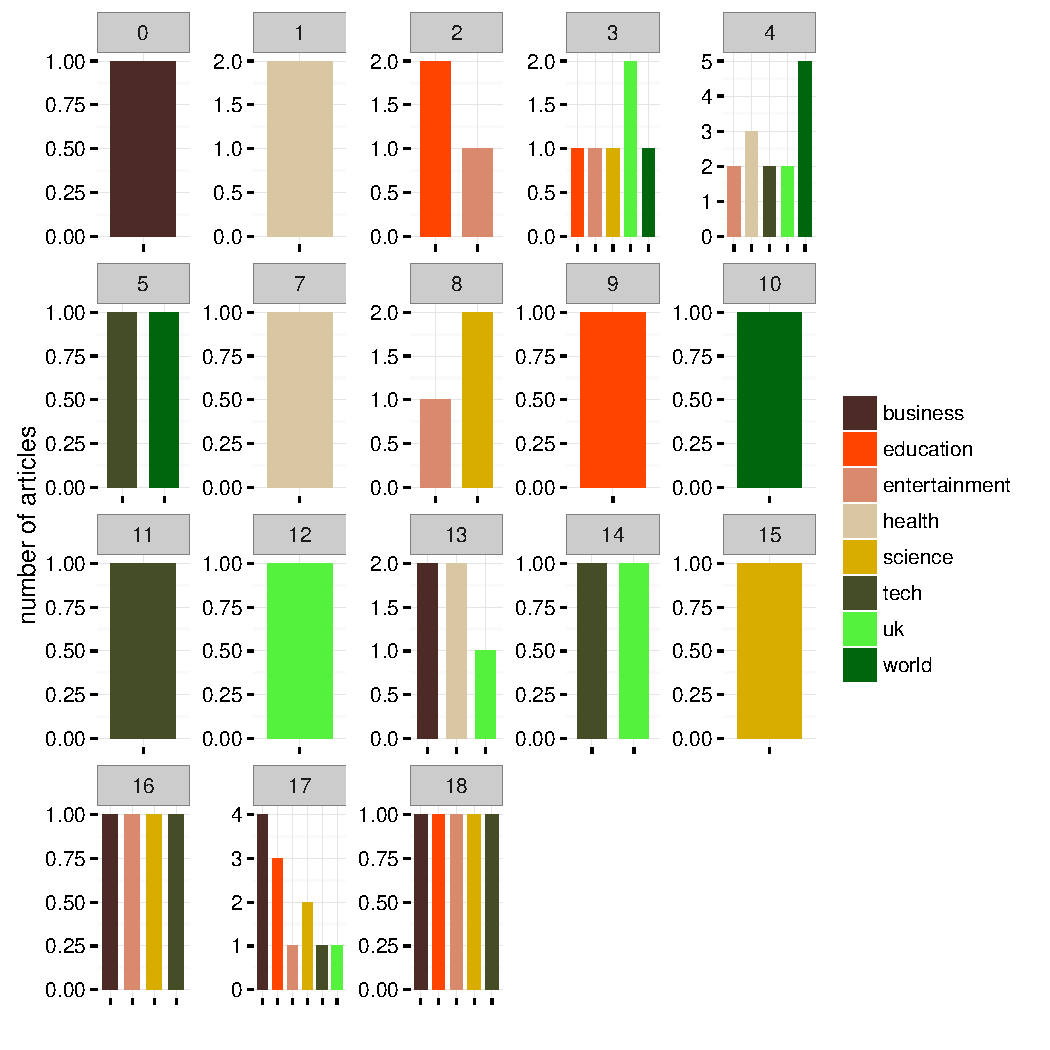
\includegraphics[width=.48\columnwidth]{figures/520datcatogery.pdf}}
\caption{\small Topic-Category distribution of DAT model for 4 different weeks, which are between 2016.01.01 to 2016.01.07, between 2016.02.12 to 2016.02.19, between 2016.03.04 to 2016.03.11 and between 2016.05.20 to 2016.05.27}
\label{fig:dattopiccategory}
\end{figure*}

Let's start with the category \textit{education}, its association with different topics at different time can be interpreted with Figure ~\ref{fig:dattopiccategory}. Its topic evolution can be shown as in Figure ~\ref{fig:dat_education_tc}.

It shows that compared to LDA model the DAT topics are more neatly and time-related. In the week of Jan 1st, we see the words of \textit{school} which appears in most of the education news at that time. the words \textit{nation, need,expect, career} are there is due to the news that \textit{the National College of Teaching and Leadership is expecting a surge of interest in the profession of teachers} \footnote{http://www.bbc.co.uk/news/education-35193600}. The reason you see \textit{islam} is because of the news that \textit{Trojan Horse scandal in Birmingham has been prohibited from teaching indefinitely}\footnote{http://www.bbc.co.uk/news/education-35226482}. You see \textit{travel} and \textit{MP} because of the news that \textit{Pupils in a primary school in Yorkshire will have to travel to another school for part of each day because of difficulties in recruiting a teacher}\footnote{http://www.bbc.co.uk/news/education-35242877}, and MPs on the Education Select Committee are warned of a deepening "crisis" in recruiting and retaining teachers.

Then in the week of Feb 12th, we use the similar way to check DAT's performance to discover topics and prevent from confusing different event news. Since there are less than 10 news about education in this week, so it is easily to envision that the words around this topic are from the news that \textit{A flagship scheme to bring ex-servicemen and women to England's classrooms has seen 28 veterans qualify as teachers since it started.}\footnote{http://www.bbc.co.uk/news/education-35595424}, \textit{Teacher shortages mean classroom support staff are doing work normally done by qualified teachers}\footnote{http://www.bbc.co.uk/news/education-35551009}, and some other news. 

Then in the week of Mar 4th, we can see from the words that the hot news event are \textit{Harvard Law School is to change its official seal, after a protest that it had links to slavery.}\footnote{http://www.bbc.co.uk/news/education-35726878}, and \textit{a proposal of national funding formula for schools, which would be introduced next year, would see budgets going straight to schools, removing local authorities from being a channel for funding.}\footnote{http://www.bbc.co.uk/news/education-35775458}. 

Lastly in the week of May 20th, some education news started to discuss on British EU referendum, and also the topic are also related to the news that \textit{Head teachers are calling on the education secretary to stop the publication of this year's primary school results in England.}\footnote{http://www.bbc.co.uk/news/education-36372304}. 


\begin{figure}[h]
\centering
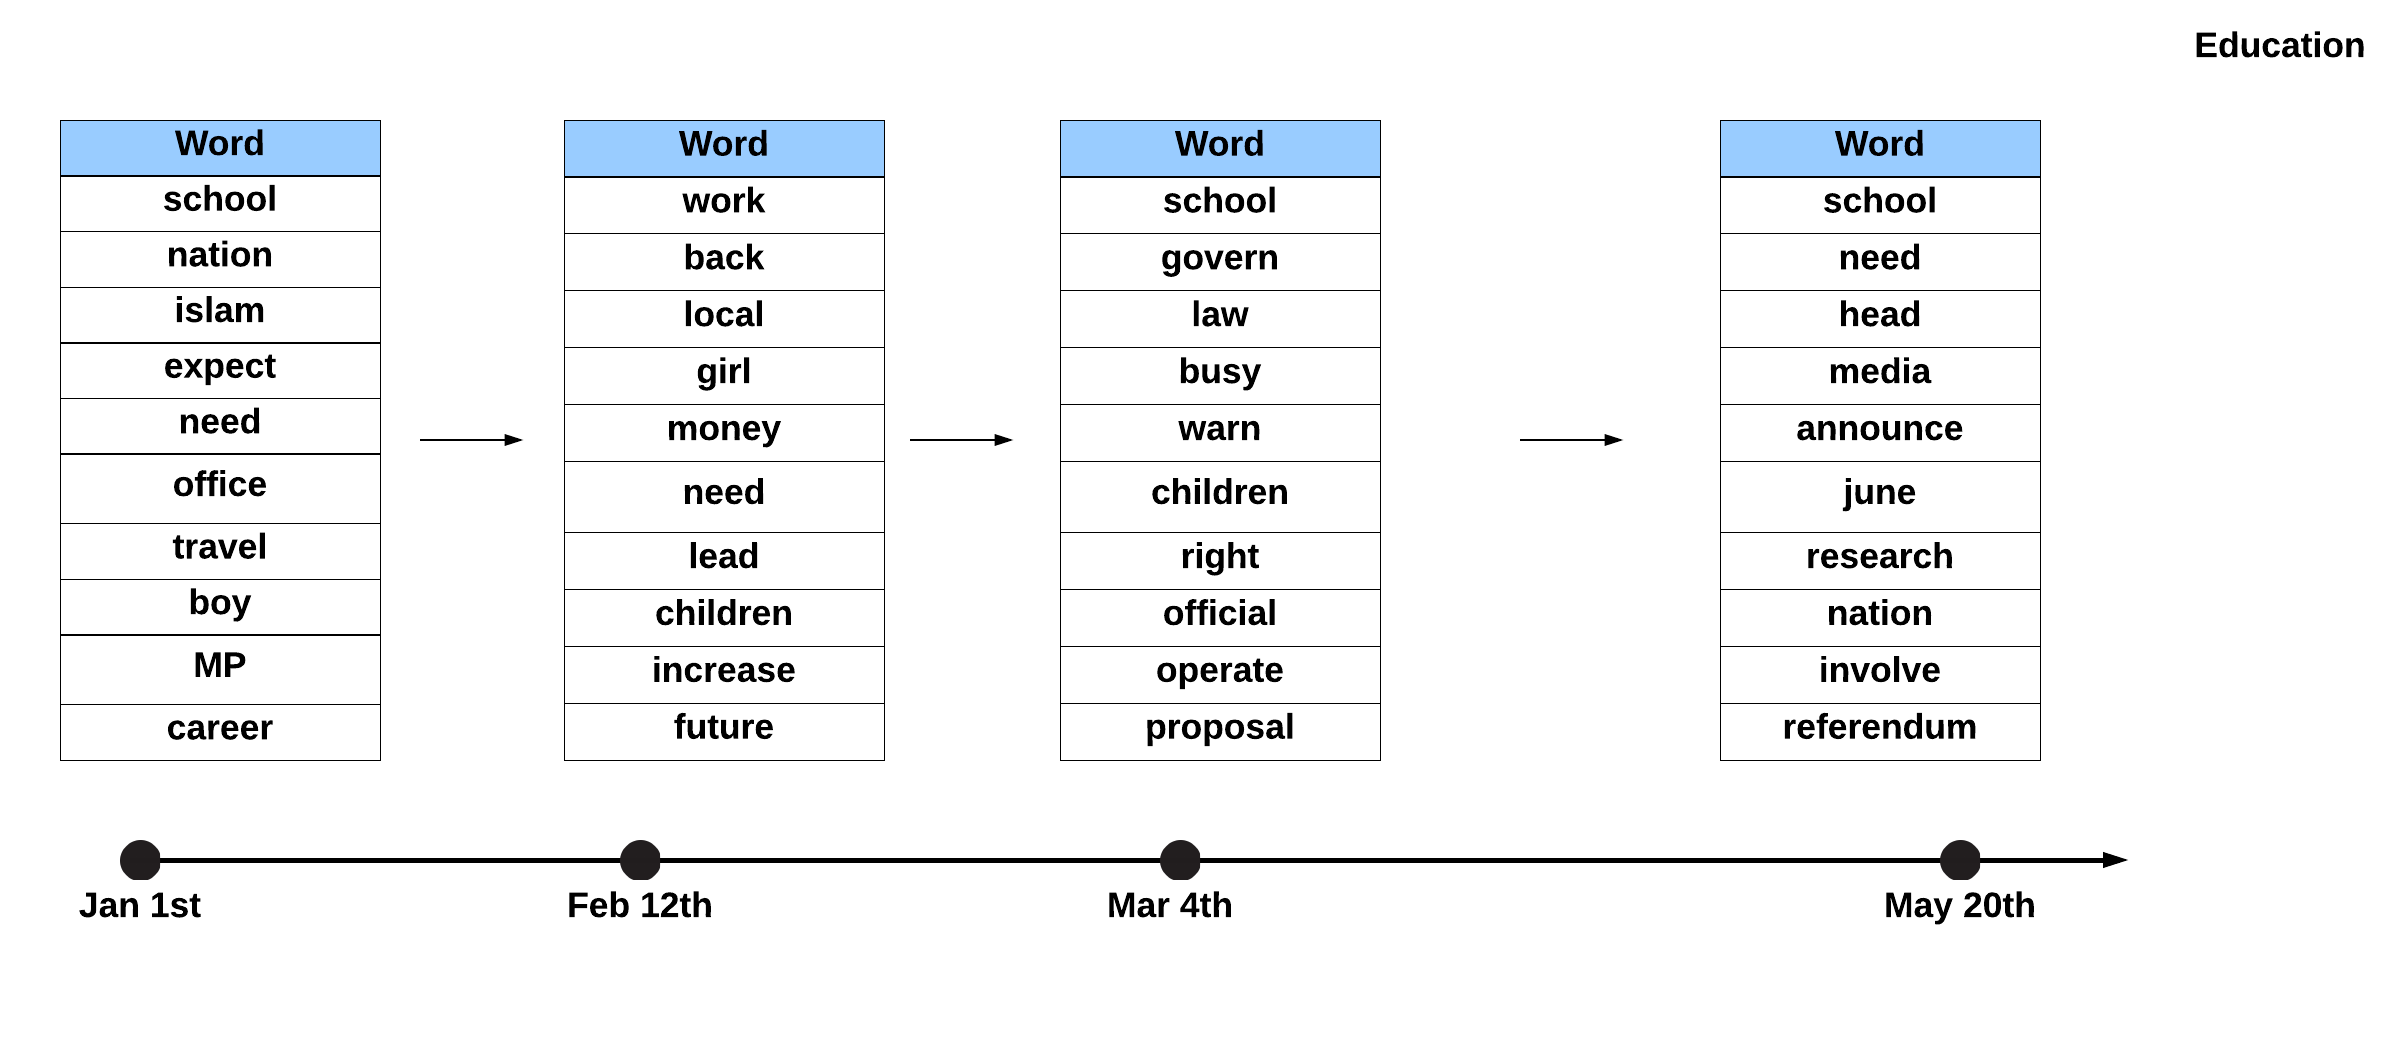
\includegraphics[width=1\textwidth]{figures/dat_education_tc.png}
\caption{Topic Evolution of DAT model: Use Education as Example}
\label{fig:dat_education_tc}
\end{figure}
\begin{figure}[h]
\centering
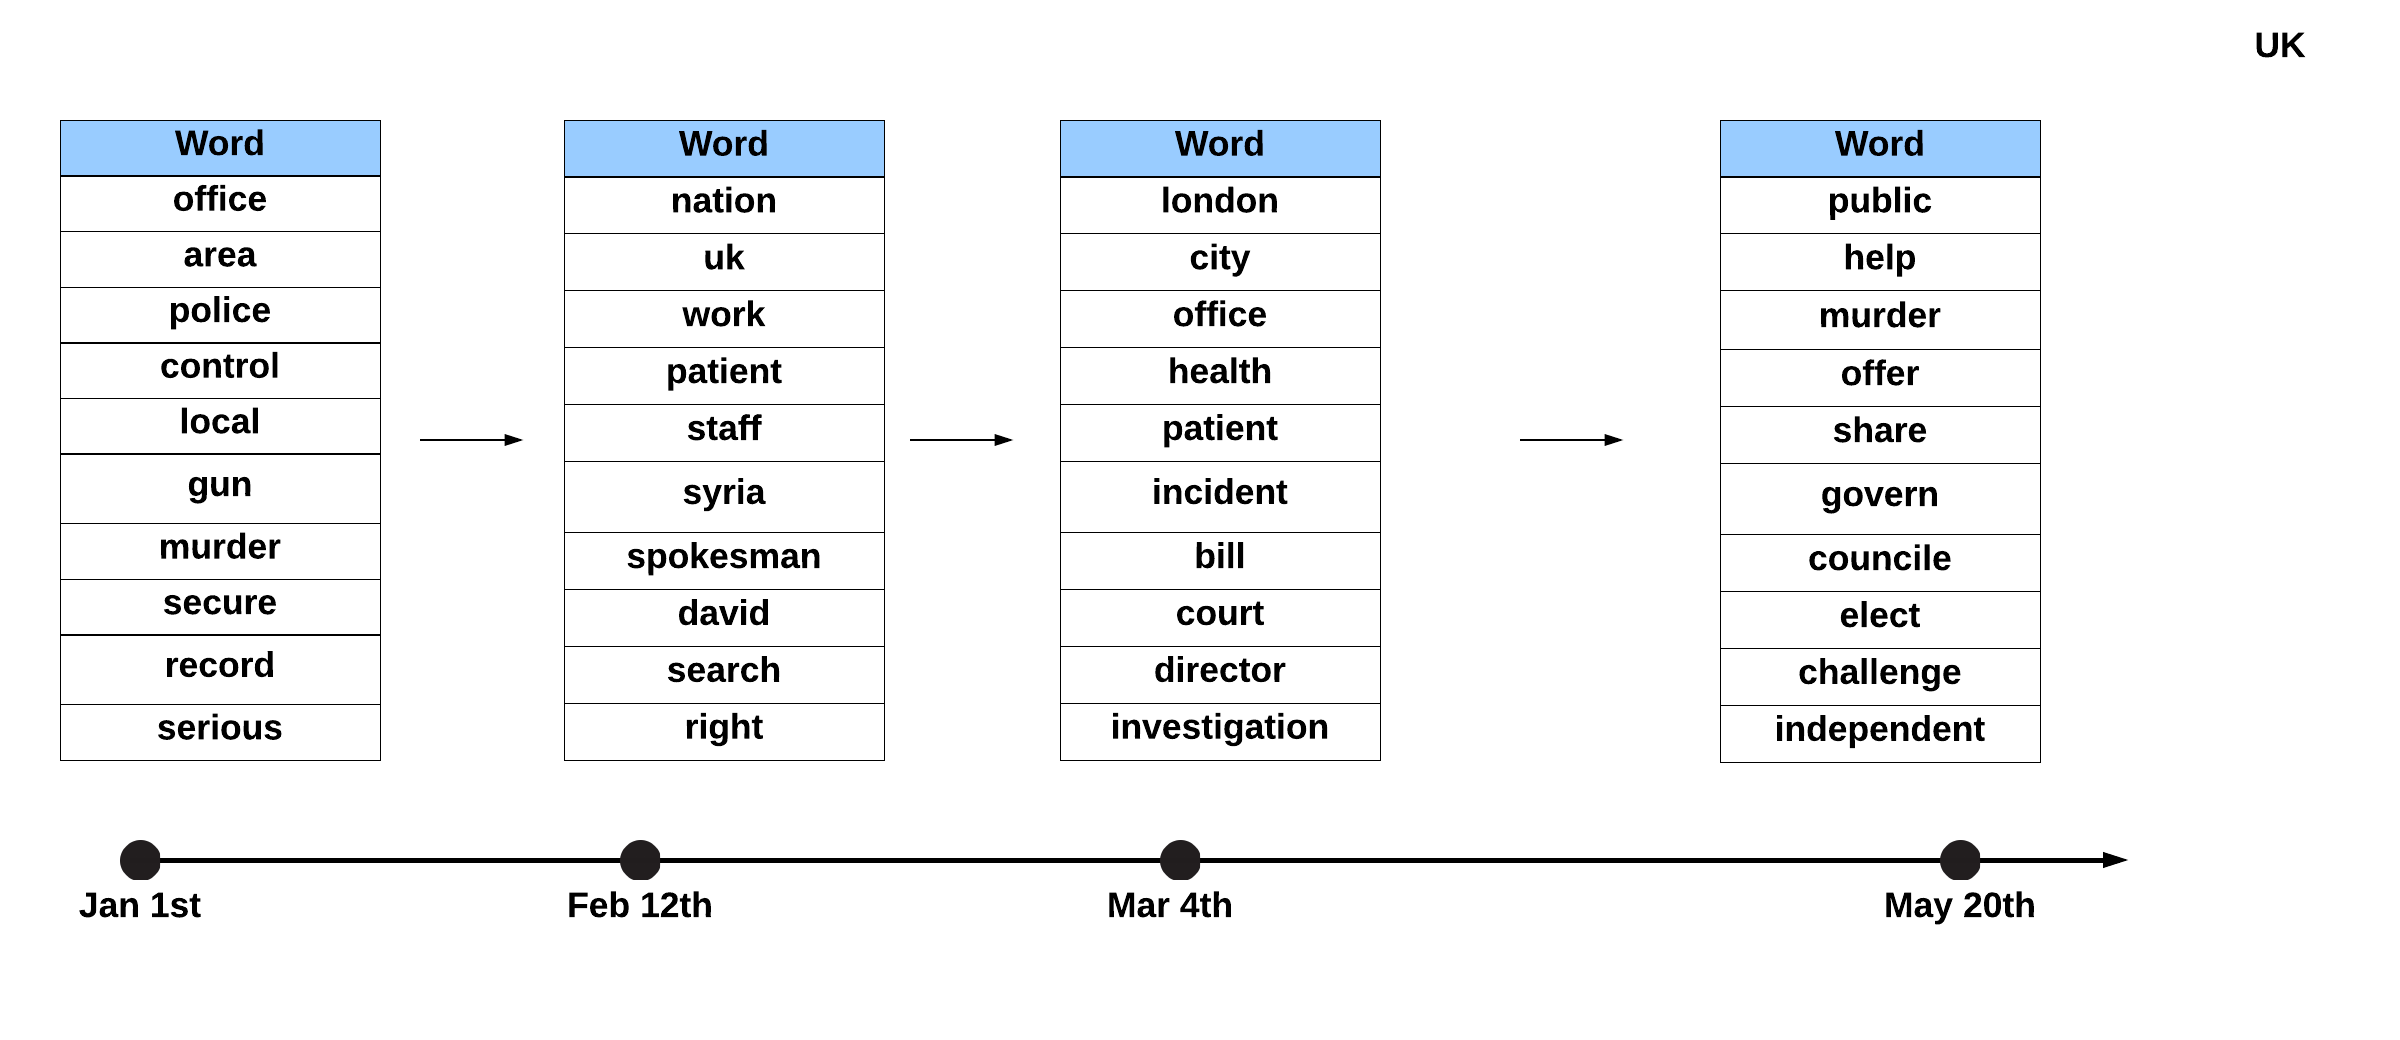
\includegraphics[width=1\textwidth]{figures/dat_uk_tc.png}
\caption{Topic Evolution of DAT model: Use UK as Example}
\label{fig:dat_uk_tc}
\end{figure}
\begin{figure}[h]
\centering
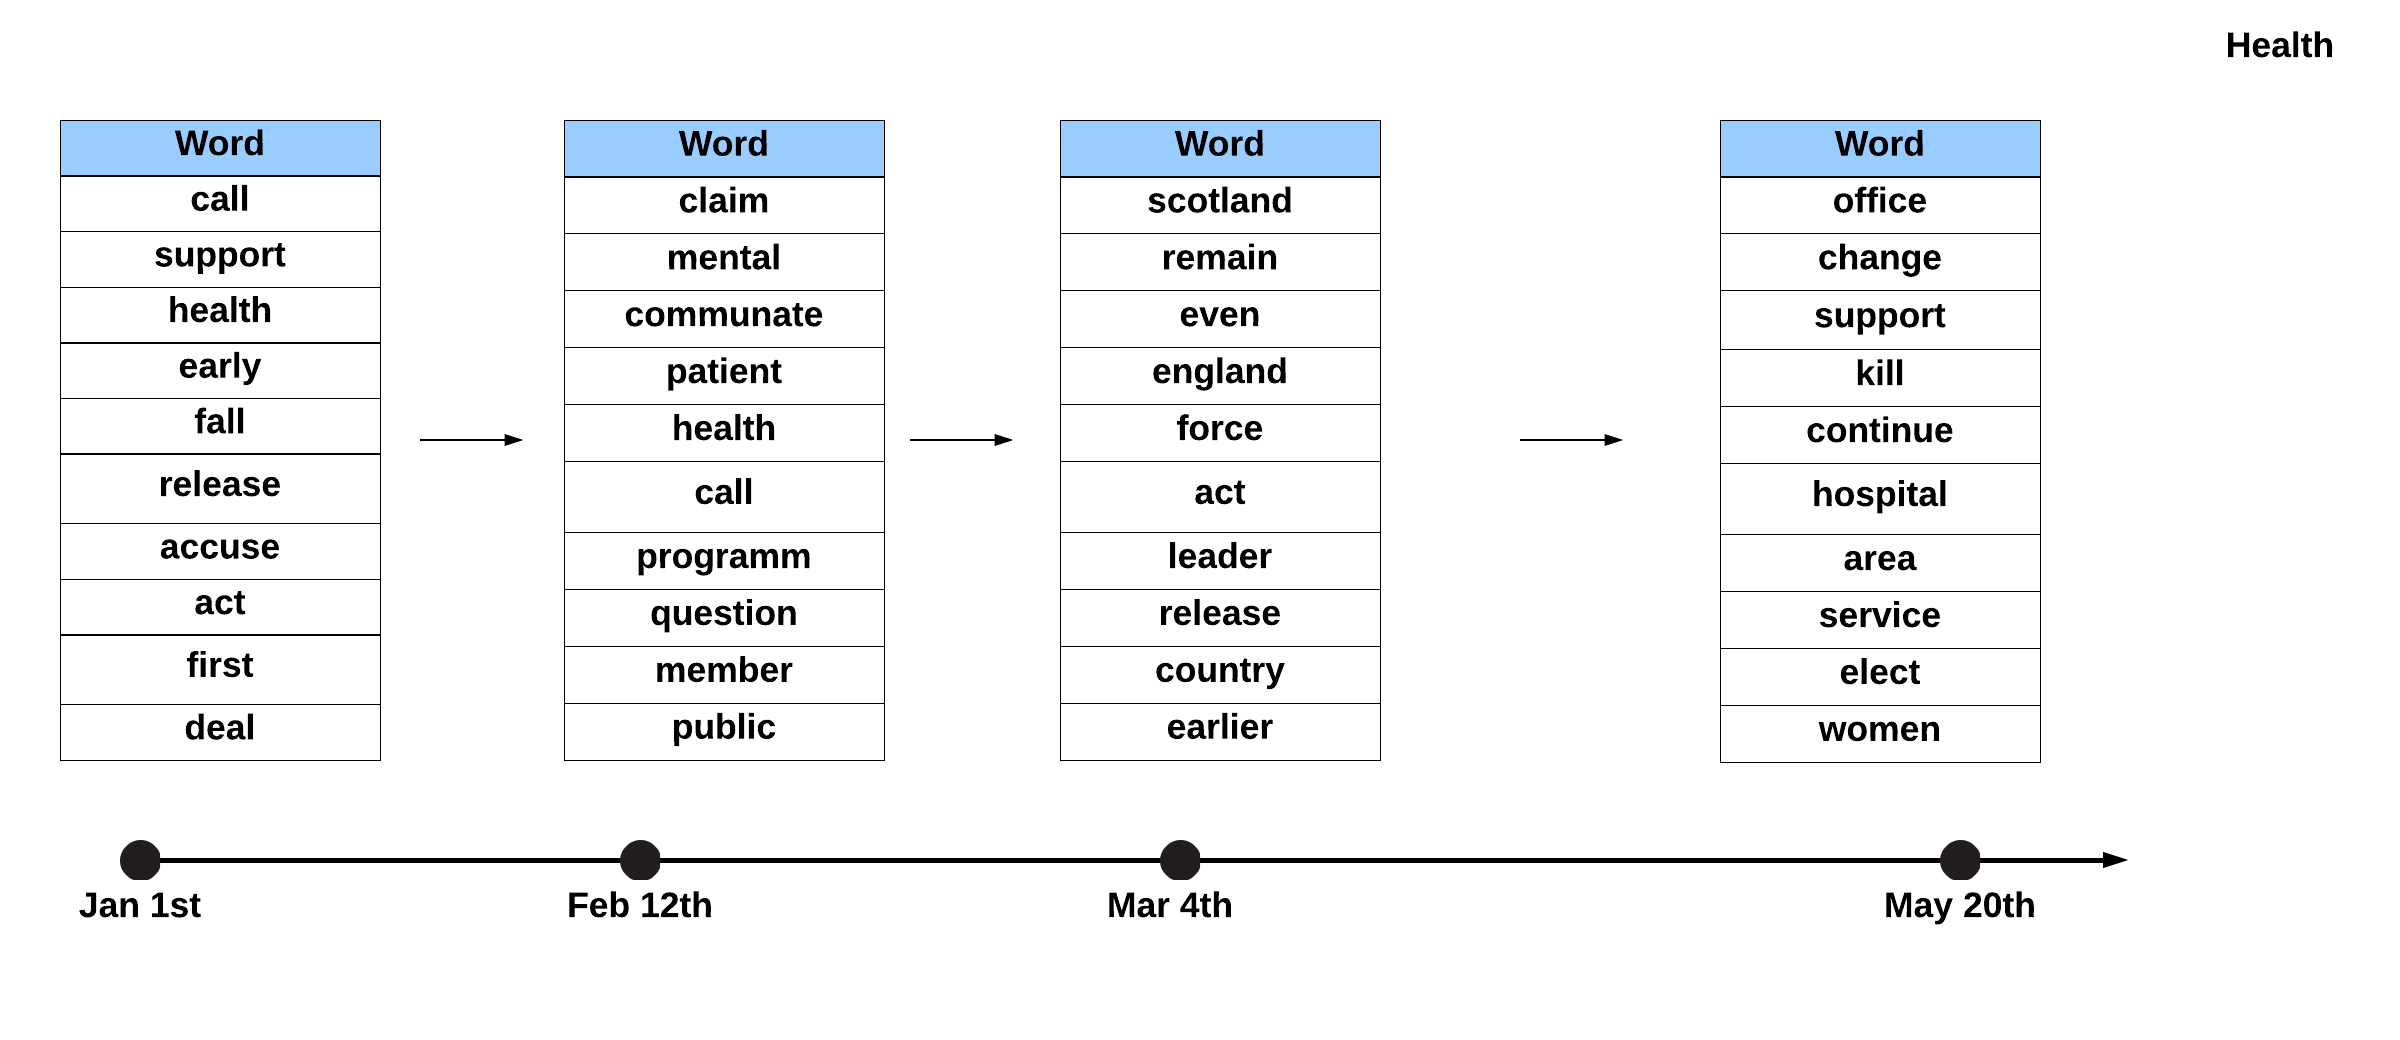
\includegraphics[width=1\textwidth]{figures/dat_health_tc.png}
\caption{Topic Evolution of DAT model: Use Health as Example}
\label{fig:dat_health_tc}
\end{figure}

Another example we can show is for category \textit{UK}, which is presented in Figure ~\ref{fig:dat_uk_tc}.

In the week of Jan 1st, quite a few news are about \textit{police, murder, secure, }, such as \textit{Man arrested over murder of Daria Pionko in Leeds}\footnote{http://www.bbc.co.uk/news/uk-england-leeds-35209489}, \textit{Pitsea stairwell death: Two men bailed by police}\footnote{http://www.bbc.co.uk/news/uk-england-essex-35209578},etc. Also we see record-breaking rainfall north-west England as the news discussed \footnote{http://www.bbc.co.uk/news/uk-england-35222030}. Then in teh week of Feb 12th, we see the news about \textit{UCL's research that a patient embodying themselves in a virtual reality avatar of a crying child could help with depression}\footnote{http://www.bbc.co.uk/news/uk-35558447}. and \textit{search on Ben Nevis for missing climbers}\footnote{http://www.bbc.co.uk/news/uk-35594715} and mostly, the Syria crisis. Then when in the week of Mar 4th, one important UK news is that \textit{One of London mayoral hopeful Sadiq Khan's aides, Shueb Salar, has resigned following his suspension on Sunday.}\footnote{http://www.bbc.co.uk/news/uk-england-london-35744843}, the news that \textit{Clayton Williams tells court he 'did not intend to kill officer'}\footnote{http://www.bbc.co.uk/news/uk-35756062}, an incident at Hyder park gate \footnote{http://www.bbc.co.uk/news/uk-england-london-35752992}, and a few investigation of criminals. \footnote{http://www.bbc.co.uk/news/uk-wales-south-east-wales-35747691}. While in the week of May 20th, we still see a few news about murder \footnote{http://www.bbc.co.uk/news/uk-england-essex-36248166} \footnote{http://www.bbc.co.uk/news/uk-england-36376555} \footnote{http://www.bbc.co.uk/news/uk-england-manchester-36375040}, \textit{the news that European countries urged to improve data sharing to improve the way they gather and share information about firearms to cut gun crime}\footnote{http://www.bbc.co.uk/news/uk-36371145}, and surely many news about election in May.

The last example is the category of \textit{health}, we only show the topic evolution here in Figure ~\ref{fig:dat_health_tc}, which also uncovered the news trends among the 5 months.


The other topics also have the same pattern of changing and evolution which can indicate the rising and falling of the topics over time. Compared to LDA model, DAT's Topic-Category distribution is not as prominent as LDA model so the topic segmentation is less clear than LDA. However, DAT obviously has the advantages that it tracks the news trends and words to describe the topics are time and event specifically, unlike for LDA model the words are mostly general words which spread through the whole news corpus's time. Also DAT will not be confused by different events and is able to identify the event-specific words for the topics. An good example is that the word \textit{Islam} appears as the one of the most relevant words for topic \textit{education} on Jan 1st. Although there is no direct relation between them however since there is a news about prohibiting Trojan Horse scandal which is hotly discussed so \textit{Islam} becomes relevant to \textit{education} in this special case.

Therefore to answer \textbf{RQ1} LDA outperforms DAT, and DAT is better for \textbf{RQ3,4} and \textbf{6}.


\section{Performance Comparison between Dynamic Author-Topic and Author-Topic Models}

In this section we will compare the performance of static Author-Topic model and the Dynamic Author-Topic model. The parameters of Author-topic model is set as $\alpha = 0.1$, $\beta = 0.01$, and the same as the number of categories of BBC news, $\text{Author Number} = 9$, and the topic number here is set as 20. The Dynamic Author-Topic model has exactly the same parameters as the static one.

\subsection{Perplexity}
The comparison of the perplexity of the two models with different number of topics is shown in Figure ~\ref{fig:at_dat_perplexity}. To answer \textbf{RQ5},Dynamic Author-Topic model's performance is improved with the increasing number of topics. However, the performance of Author-Topic model stay unchanged which is because the expectation that answer will match its previous output of its author limit its predictive power of the author-topic model since actually no two news are exactly the same. The authorship information does not contribute to the predictive capability of AT model in this case since we the 9 authors we have are virtual ones with no valid meaning. The writing styles of the news from category \textit{UK} and \textit{education} are overlapped and confused between each other. So the authorship are somewhat randomly assigned to the word tokens for AT model. Our proposed model is adaptive to the changing writing styles of the news so that the randomness is removed to some extent. To answer \textbf{RQ6}, DAT has much better topic generalization performance than AT model.

\begin{figure}[h]
\centering
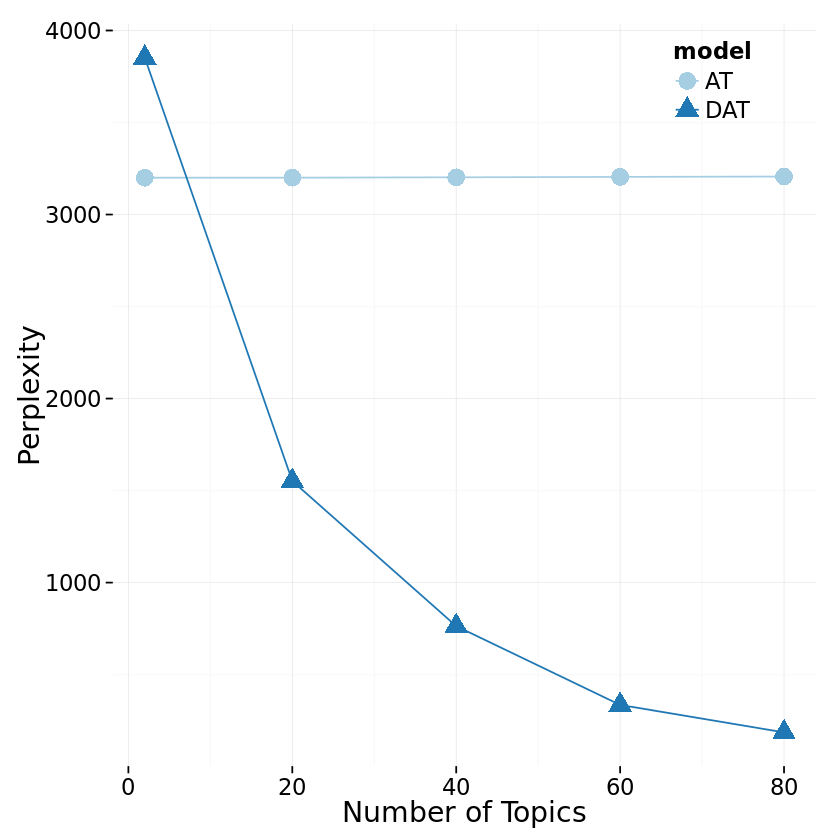
\includegraphics[width=1\textwidth]{figures/at_dat_perplexity.png}
\caption{Mean perplexity of DAT and AT with varying numbers of latent topics.}
\label{fig:at_dat_perplexity}
\end{figure}

\subsection{Topic Distribution}


Similar to Table ~\ref{table:ldatopicdistribution}, here we have shown the examples of 6 topics with author information, but here due to space limitation we only show the top 10 most likely words to be generated conditioned on the topic, and 4 top most likely authors to have generated a word conditioned on the topic. The topic-category distribution of the Author-Topic model is shown in Figure ~\ref{fig:at_topic_category}. And our interpreting of the topic as well its words distribution can be shown in Table ~\ref{table:at_topic_distribution}. 

\begin{figure}[h]
\centering
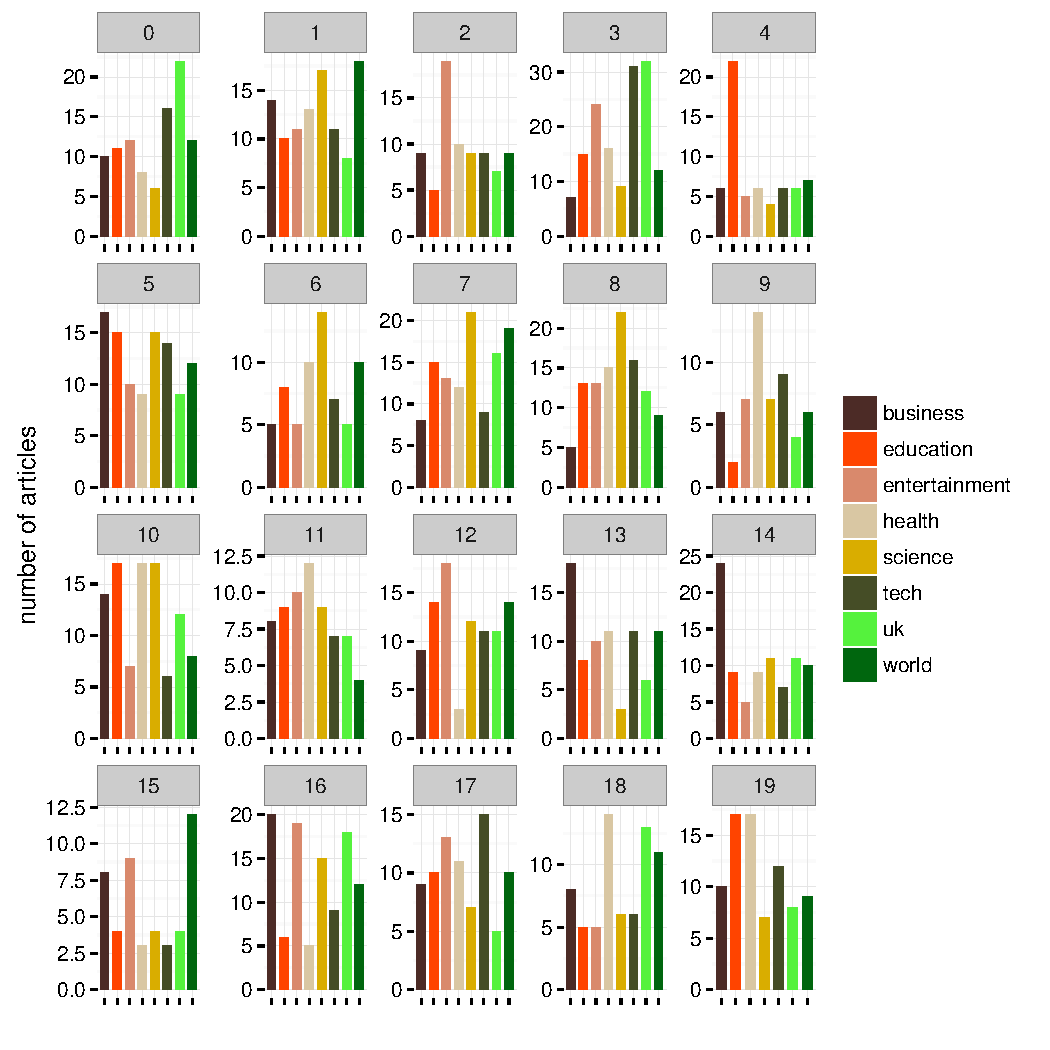
\includegraphics[width=1\textwidth]{figures/at_topic_category.pdf}
\caption{Topic-Categoy distribution of Author-Topic model.}
\label{fig:at_topic_category}
\end{figure}


\begin{table}[h!]
\centering
\begin{tabular}{|c c|} 
\hline
\multicolumn{2}{|c|}{\textbf{Topic 0 : UK}} \\
\hline
 \textbf{WORD} & \textbf{PROB}.  \\ [0.3ex] 
 \hline
 	police  &   0.011306\\
	expect   &  0.007149\\
	attack  &   0.005665\\
	cause  &   0.005397\\
	site  &   0.004464\\
	put   &  0.004408\\
	road   &  0.004307\\
	country  &   0.004144\\
	investigation  &   0.004074\\
	foreign   &  0.003674\\[1ex] 
 \hline
  \textbf{AUTHOR} & \textbf{PROB}.  \\ [0.3ex] 
 \hline
 6  & 0.12136\\
8  &   0.11783\\
5  &   0.11711\\
3  &   0.11258\\
 \hline
\end{tabular}
 \hfill
\begin{tabular}{|c c|} 
\hline
\multicolumn{2}{|c|}{\textbf{Topic 2 : Entertainment}} \\
\hline
 \textbf{WORD} & \textbf{PROB}.  \\ [0.3ex] 
 \hline
 	place  & 0.004633 \\
 	shot   & 0.004466\\
	first  &  0.004243\\
	close  &  0.004184\\
	facebook  &  0.004080\\
	well   &    0.003947\\
	become    &   0.003857\\
	look   &    0.003819\\
	improve   &    0.003753\\
	side    &   0.003694\\[1ex] 
 \hline
  \textbf{AUTHOR} & \textbf{PROB}.  \\ [0.3ex] 
 \hline
 7  & 0.12367\\
4   &  0.11519\\
2  &   0.11368\\
3  &   0.11360\\
 \hline
\end{tabular}
 \hfill
 \begin{tabular}{|c c|} 
\hline
\multicolumn{2}{|c|}{\textbf{Topic 4 : Education}} \\
\hline
 \textbf{WORD} & \textbf{PROB}.  \\ [0.3ex] 
 \hline
 part  & 0.006973 \\
	girl  &  0.005364\\
	man   & 0.005104\\
	read  &  0.004729\\
	school  &  0.004672\\
	appeal   & 0.004640\\
	parent   & 0.004473\\
	reveal  &  0.004416\\
	go   & 0.004294\\
	public  &  0.004241 \\ [1ex] 
 \hline
  \textbf{AUTHOR} & \textbf{PROB}.  \\ [0.3ex] 
 \hline
 0  & 0.12073 \\ 
1   &  0.11673 \\ 
4  &   0.11618 \\ 
7  &   0.112373 \\ 
 \hline
\end{tabular}
\hfill
\\[1cm]
\begin{tabular}{|c c|} 
\hline
\multicolumn{2}{|c|}{\textbf{Topic 14 : Business}} \\
\hline
 \textbf{WORD} & \textbf{PROB}.  \\ [0.3ex] 
 \hline
 many &  0.005329 \\ 
	like  &    0.005039 \\ 
	need   &   0.004944 \\ 
	month  &    0.004247 \\ 
	made  &    0.004159 \\ 
	charge  &    0.004054 \\ 
	make  &    0.003994 \\ 
	price  &    0.003814 \\ 
	case  &    0.003686 \\ 
	union  &    0.003612 \\ [1ex] 
 \hline
  \textbf{AUTHOR} & \textbf{PROB}.  \\ [0.3ex] 
 \hline
 7 &  0.12653 \\
3 &   0.11960 \\
5 &   0.11089 \\
2 &   0.11010  \\
 \hline
 \end{tabular} 
\hfill
 \begin{tabular}{|c c|} 
\hline
\multicolumn{2}{|c|}{\textbf{Topic 15 : World}} \\
\hline
 \textbf{WORD} & \textbf{PROB}.  \\ [0.3ex] 
 \hline
 live  & 0.005703\\ 
	die   &  0.004945\\ 
	ahead  &   0.004934\\ 
	man   &  0.004902\\ 
	govern  &   0.004725\\ 
	tax   &  0.004625\\ 
	author  &   0.004103\\ 
	hope   &  0.004006\\ 
	member  &   0.003923\\ 
	conservative  &   0.003762\\ [1ex] 
 \hline
  \textbf{AUTHOR} & \textbf{PROB}.  \\ [0.3ex] 
 \hline
 3 &   0.11515 \\
4  &    0.11366 \\
5   &   0.11247 \\
0  &    0.11227  \\
 \hline
 \end{tabular} 
\hfill
\begin{tabular}{|c c|} 
\hline
\multicolumn{2}{|c|}{\textbf{Topic 18 : Health}} \\
\hline
 \textbf{WORD} & \textbf{PROB}.  \\ [0.3ex] 
 \hline
 state &  0.006794 \\ 
	announce  &   0.005624 \\ 
	head  &   0.004991 \\ 
	govern &    0.004573 \\ 
	case &    0.004527 \\ 
	health &    0.004502 \\ 
	number &    0.004211 \\ 
	country&    0.004123 \\ 
	shop  &   0.003961 \\ 
	council &  0.003655 \\ [1ex] 
 \hline
  \textbf{AUTHOR} & \textbf{PROB}.  \\ [0.3ex] 
 \hline
 7 &  0.12653 \\
3 &   0.11960 \\
5 &   0.11089 \\
2 &   0.11010  \\
 \hline
 \end{tabular} 
\hfill
\caption{Author-Topic model Topic Distribution}
\label{table:at_topic_distribution}
\end{table}

We can see that the authorship is evenly distributed over the topics which means the authorship information is not very useful in our case since the authors' contribution for each topic can not be differentiated easily. The reason is that our 9 authors are virtually set and our expectation that the news in different categories are different has limited the flexibility of the topic assignment of the DAT model. To compare we have selected the BBC news published in the week of May 6th (which is different from the weeks in Section ~\ref{sec:ldadat}). We can see that the word distribution for DAT model is more specific and the author distribution is more diverse than AT model.  


\begin{table}[h!]
\centering
\begin{tabular}{|c c|} 
\hline
\multicolumn{2}{|c|}{\textbf{Topic 0 : UK}} \\
\hline
 \textbf{WORD} & \textbf{PROB}.  \\ [0.3ex] 
 \hline
 	party &  0.029783\\
	conserve  &   0.020655\\
	chief  &   0.018636\\
	industry  &   0.018239\\
	parliament  &   0.014519\\
	role  &   0.013771\\
	allow  &   0.012798\\
	leave  &   0.012498\\
	challenge   &  0.012423\\
	secretary   &  0.012295\\[1ex] 
 \hline
  \textbf{AUTHOR} & \textbf{PROB}.  \\ [0.3ex] 
 \hline
 2 &  0.12066\\
1  & 0.11389\\
5  & 0.10803\\
6  & 0.098594\\
 \hline
\end{tabular}
 \hfill
\begin{tabular}{|c c|} 
\hline
\multicolumn{2}{|c|}{\textbf{Topic 4 : World}} \\
\hline
 \textbf{WORD} & \textbf{PROB}.  \\ [0.3ex] 
 \hline
 	police &  0.054837\\
	state &   0.025174\\
	area &   0.022276\\
	party &   0.018467\\
	elect &   0.016934\\
	trade &   0.015518\\
	trump &   0.014928\\
	power &   0.014887\\
	provide &   0.014036\\
	uk &   0.013866\\[1ex] 
 \hline
  \textbf{AUTHOR} & \textbf{PROB}.  \\ [0.3ex] 
 \hline
0 &  0.12009\\
2 &  0.11484\\
1 &  0.11441\\
5  & 0.10904\\
 \hline
\end{tabular}
 \hfill
 \begin{tabular}{|c c|} 
\hline
\multicolumn{2}{|c|}{\textbf{Topic 9 : Education}} \\
\hline
 \textbf{WORD} & \textbf{PROB}.  \\ [0.3ex] 
 \hline
 support &  0.023740\\
	make  &    0.022040\\
	family   &   0.016543\\
	assemble  &   0.015807\\
	school   &   0.015694\\
	children  &    0.015580\\
	site   &   0.015215\\
	injury   &   0.014731\\
	cost   &   0.013979\\
	help   &   0.013598\\ [1ex] 
 \hline
  \textbf{AUTHOR} & \textbf{PROB}.  \\ [0.3ex] 
 \hline
 6 &  0.11991 \\ 
4  &    0.11339\\
2  &    0.11301\\
8  &    0.11194 \\ 
 \hline
\end{tabular}
\hfill
\\[1cm]
\begin{tabular}{|c c|} 
\hline
\multicolumn{2}{|c|}{\textbf{Topic 15 : UK Politics}} \\
\hline
 \textbf{WORD} & \textbf{PROB}.  \\ [0.3ex] 
 \hline
	world &  0.023130\\
	london &   0.019875\\
	south &   0.019585\\
	product &   0.017882\\
	elect &   0.016504\\
	vote &   0.016387\\
	finance &   0.015132\\
	depart &   0.014511\\
	agency &   0.013886\\
	david &   0.012805\\ [1ex] 
 \hline
  \textbf{AUTHOR} & \textbf{PROB}.  \\ [0.3ex] 
 \hline

4 &  0.11802\\
8  &   0.11681\\
1   &  0.11148\\
2   &  0.11089\\
 \hline
 \end{tabular} 
\hfill
 \begin{tabular}{|c c|} 
\hline
\multicolumn{2}{|c|}{\textbf{Topic 16 : Health}} \\
\hline
 \textbf{WORD} & \textbf{PROB}.  \\ [0.3ex] 
 \hline
	health  & 0.020498\\
	change  &  0.020243\\
	company  &  0.019476\\
	road   & 0.017493\\
	care  &  0.01701\\
	woman &   0.014633\\
	import  &  0.014289\\
	england   & 0.014035\\
	hospital  &  0.013980\\
	claim  &  0.013552\\ [1ex] 
 \hline
  \textbf{AUTHOR} & \textbf{PROB}.  \\ [0.3ex] 
 \hline
 3 &  0.11886\\
5  &   0.11264\\
1  &   0.11230\\
8  &   0.10943  \\
 \hline
 \end{tabular} 
\hfill
\begin{tabular}{|c c|} 
\hline
\multicolumn{2}{|c|}{\textbf{Topic 18 : Business}} \\
\hline
 \textbf{WORD} & \textbf{PROB}.  \\ [0.3ex] 
 \hline
 service &  0.029095 \\
	issue &     0.025055 \\
	held   &   0.020426 \\
	help   &   0.020279 \\
	investigation &     0.017410 \\
	event   &   0.016605 \\
	ad   &   0.016459 \\
	former  &    0.016311 \\
	leave   &   0.016091 \\
	prime &     0.014764 \\ [1ex] 
 \hline
  \textbf{AUTHOR} & \textbf{PROB}.  \\ [0.3ex] 
 \hline
5  & 0.11912\\
0   &  0.11677 \\
3  &   0.11633\\
8  &   0.11203  \\
 \hline
 \end{tabular} 
\hfill
\caption{Dynamic Author-Topic model Topic Distribution, on May 6th}
\label{table:datat_topic_distribution}
\end{table}


We also see that the words generated for each topic using AT model is also general as LDA model. To answer \textbf{RQ1,3,4}, by comparing with our experimental results in Section \ref{sec:ldadat} definitely DAT works much better than AT model.


\section{Performance Comparison between Dynamic Author-Topic and Dynamic Topic Models}
\subsection{Perplexity}
\subsection{Topic Distribution}

Compared with Figure \ref{fig:dattopiccategory}

\begin{figure*}[!t]
  \centering
    \subfigure[2016.01.01 to 2016.01.07]{
    \label{subfig:11dattopiccategory} 
    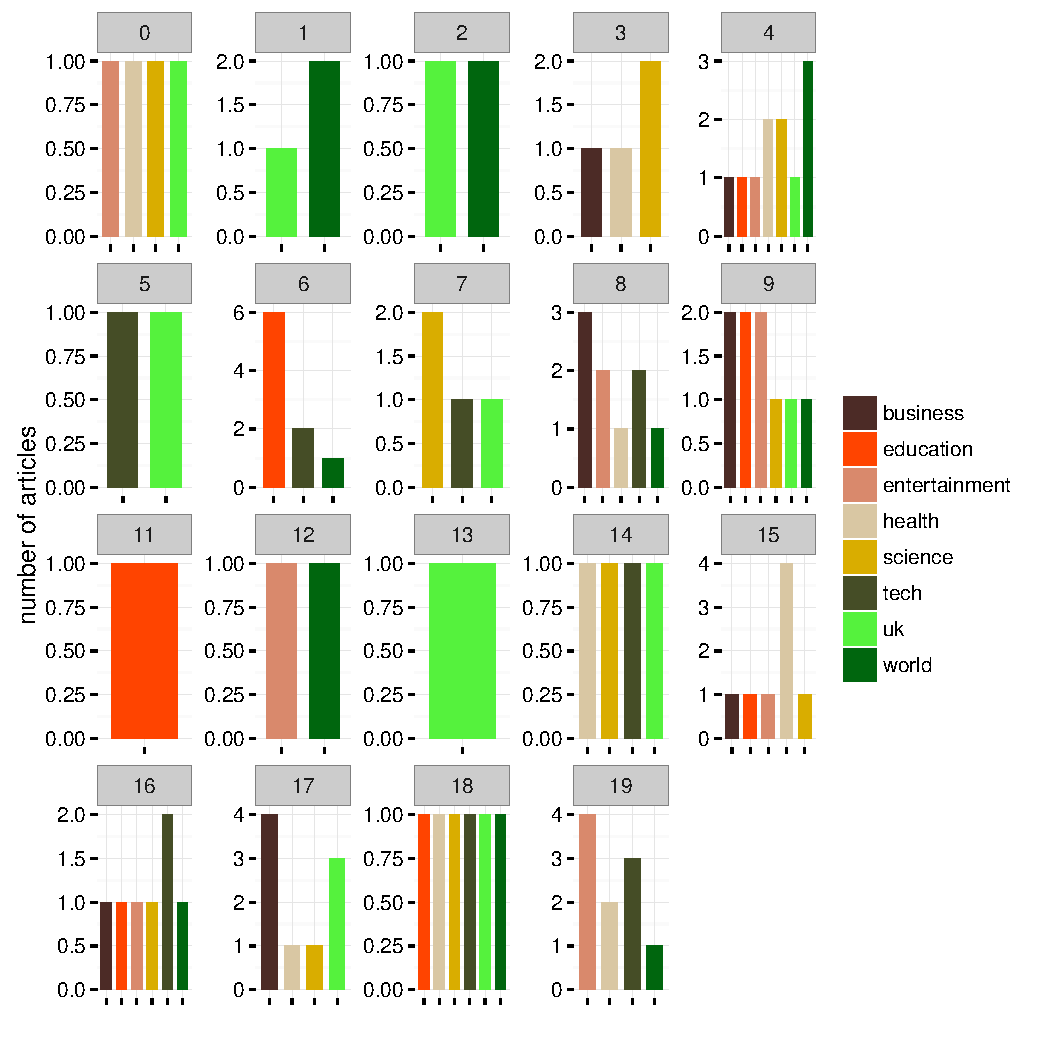
\includegraphics[width=.48\columnwidth]{figures/11datcatogery.pdf}}
    \subfigure[2016.02.12 to 2016.02.19]{
    \label{subfig:212dattopiccategory} 
    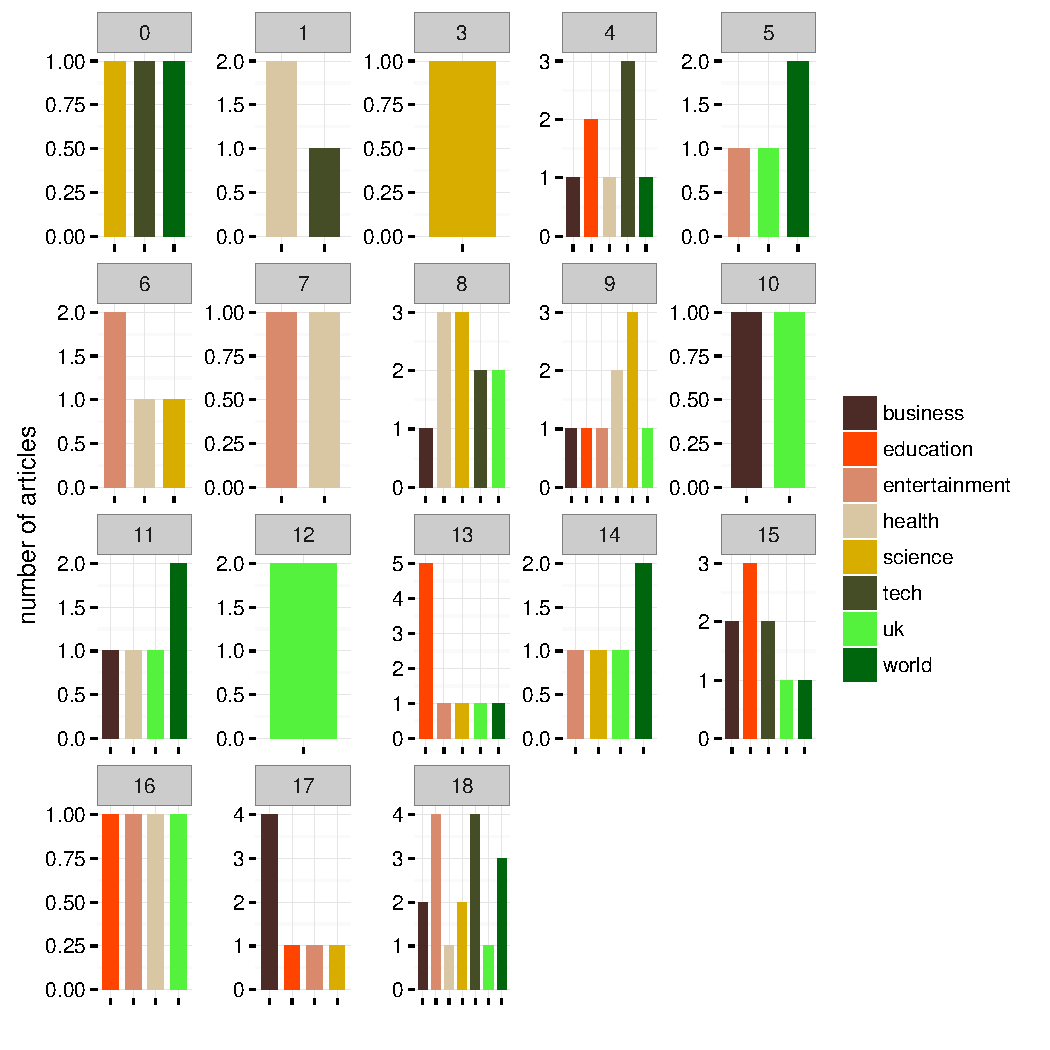
\includegraphics[width=.48\columnwidth]{figures/212datcatogery.pdf}}
    \vspace*{-.9\baselineskip}
    \subfigure[2016.03.04 to 2016.03.11]{
    \label{subfig:34dattopiccategory} 
    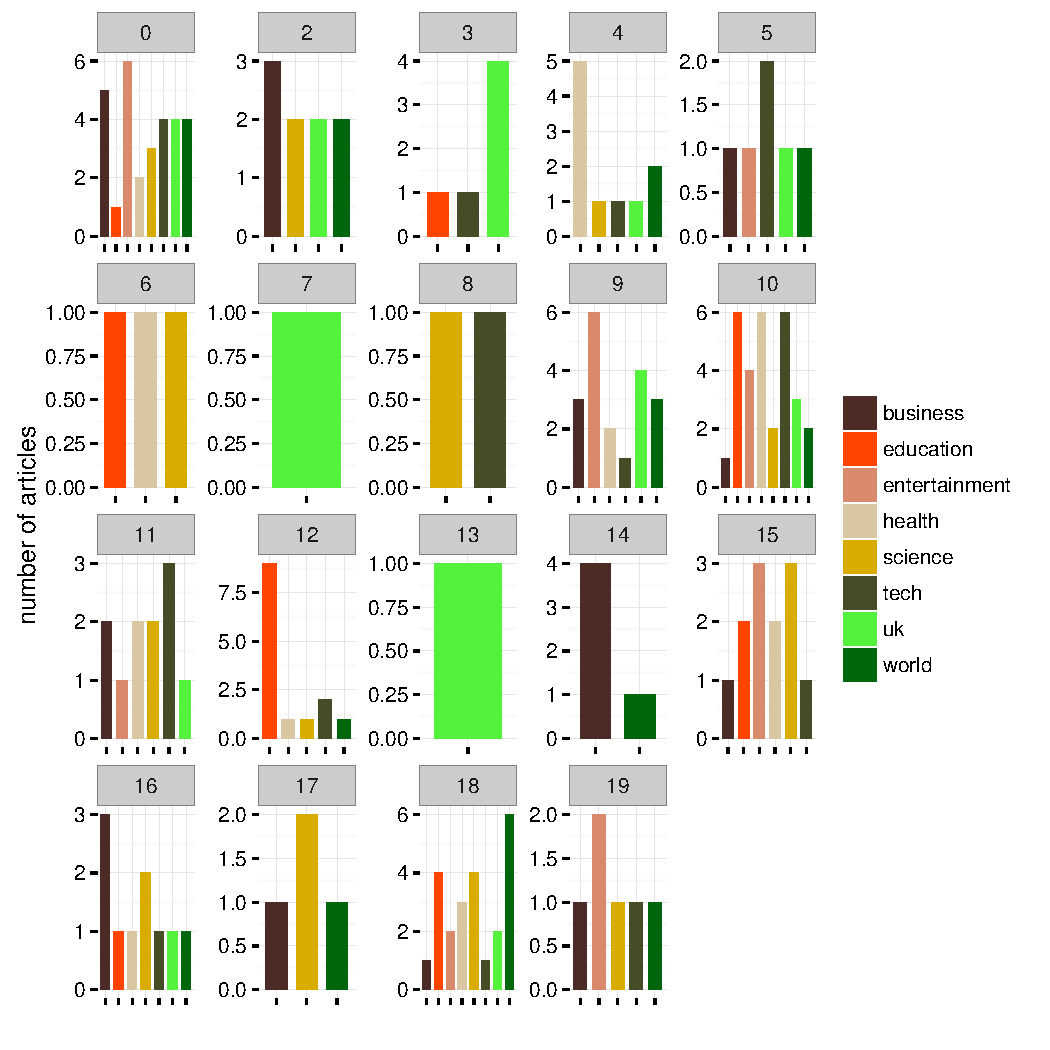
\includegraphics[width=.48\columnwidth]{figures/34datcatogery.pdf}}
    \subfigure[2016.05.20 to 2016.05.27]{
    \label{subfig:520dattopiccategory} 
    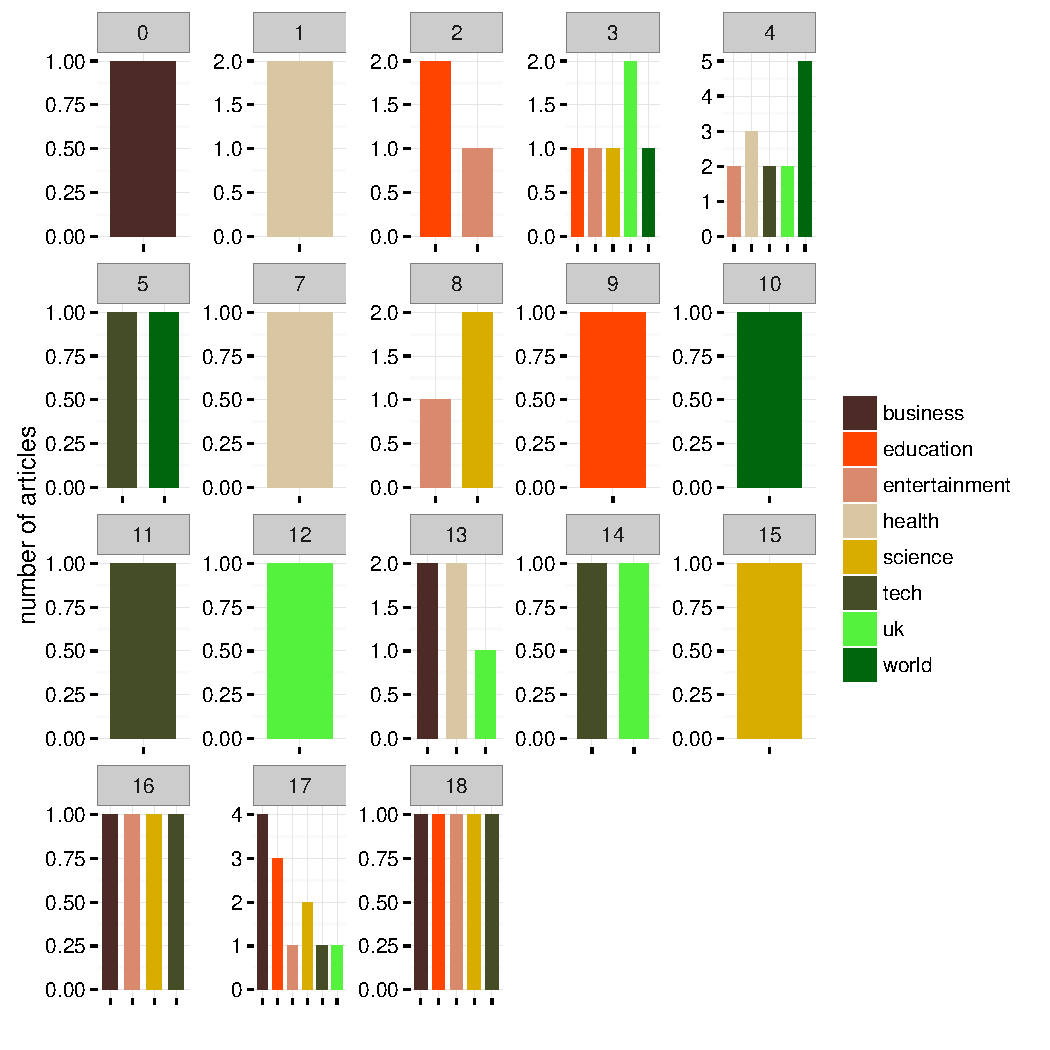
\includegraphics[width=.48\columnwidth]{figures/520datcatogery.pdf}}
\caption{\small Topic-Category distribution of TTM model for 4 different weeks, which are between 2016.01.01 to 2016.01.07, between 2016.02.12 to 2016.02.19, between 2016.03.04 to 2016.03.11 and between 2016.05.20 to 2016.05.27}
\label{fig:tottopiccategory}
\end{figure*}

\section{Comprehensive Comparison}
Based on our experiments in Section 5.1 to 5.3, we can answer our research questons as follows,
\begin{description}
	\item On the basis of classification performance:
	\begin{description}
	\item[\textbf{RQ1}:] How does the proposed DAT model perform compared to baseline algorithms in terms of topic extraction? %(See Section~\ref{subsec:diversification})
	\item[\textbf{RQ2}:] How does the performance of the DAT model change with varying length of dependency time ?
	\item[\textbf{RQ3}:] How does the proposed DAT model perform in terms of topic evolution? %(See Section~\ref{})
	\item[\textbf{RQ4}:] How does the proposed DAT model perform in terms of preventing from confounding co-occurrence patterns for topic discovery? %(See Section~\ref{})
	\item[\textbf{RQ5}:] Is the performance of DAT model sensitive to the number of topics used in the model? %(See Section~\ref{}) 
	\end{description}
	\item On the basis of the generative model:
	\begin{description}
	\item[\textbf{RQ6}:] What is the performance of the generative DAT model compared to other baseline topic models in terms of the likelihood of generating the news document measured by perplexity as discussed in Section ~\ref{sec:perpelexity}?
	\end{description}
\end{description}
\subsection{Perplexity}
\subsection{Topic Distribution}




\section{Performance with Different Time Slices}


% This just dumps some pseudolatin in so you can see some text in place.
\subsection{Topic Distribution}
In this part in order to compare to the results in Figure ~\ref{fig:dat_health_tc}, ~\ref{fig:dat_uk_tc} and \ref{fig:dat_education_tc}, we will show the topic evolution for topic \textit{health, education} and \textit{UK}. The topic number here is set as 20. 

When news dependency term is two week, namely half a month, we show the topic evolution of topic \textit{health} in Table ~\ref{dat_2_health_evoluation}.

The topic evolution of topic \textit{UK} is in Table \ref{dat_2_uk_evoluation}. 

The topic evolution of topic \textit{Education} is in Table \ref{dat_2_educatoin_evoluation}.

When news dependency term is four weeks, namely a month, we show the topic evolution of topic \textit{health} in Table ~\ref{dat_4_health_evoluation}.

The topic evolution of topic \textit{UK} is in Table \ref{dat_4_uk_evoluation}. 

The topic evolution of topic \textit{Education} is in Table \ref{dat_4_educatoin_evoluation}.

It can be obviously seen that with the increasing of the length of time dependency, the words to describe the topic becomes more general and the the model starts to confound the news event happening in one time period.

\begin{table}
\caption{Topic Distribution Evolution for Topic Health.(2 weeks as a time unit)}
\centering
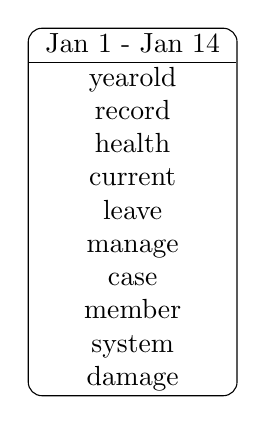
\begin{tikzpicture}
\node (table) [inner sep=0pt] {
\begin{tabular}{c}
  {Jan 1 - Jan 14} \\
  \hline
  yearold\\
	record \\
	health  \\
	current  \\
	leave  \\
	manage \\
	case \\
	member \\
	system  \\
	damage \\
\end{tabular}  
};
\draw [rounded corners=.5em] (table.north west) rectangle (table.south east);
\end{tikzpicture}
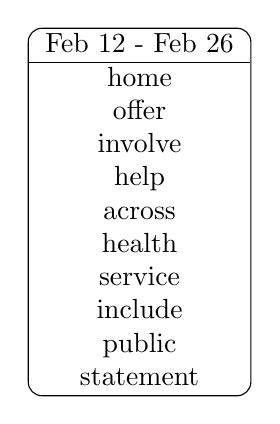
\begin{tikzpicture}
\node (table) [inner sep=0pt] {
\begin{tabular}{c}
{Feb 12 - Feb 26} \\
  \hline
 home  \\
	offer  \\
	involve \\
	help   \\
	across   \\
	health   \\
	service  \\
	include   \\
	public   \\
	statement \\
\end{tabular}
};
\draw [rounded corners=.5em] (table.north west) rectangle (table.south east);
\end{tikzpicture}
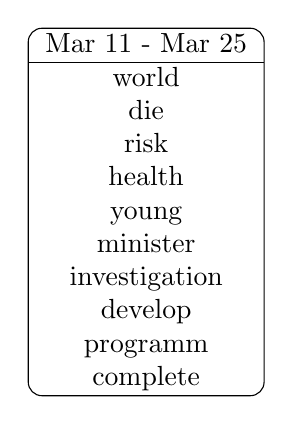
\begin{tikzpicture}
\node (table) [inner sep=0pt] {
\begin{tabular}{c}
{Mar 11 - Mar 25} \\
  \hline
 world   \\
	die   \\
	risk  \\
	health   \\
	young   \\
	minister  \\
	investigation   \\
	develop   \\
	programm   \\
	complete   \\
	
\end{tabular}
};
\draw [rounded corners=.5em] (table.north west) rectangle (table.south east);
\end{tikzpicture}
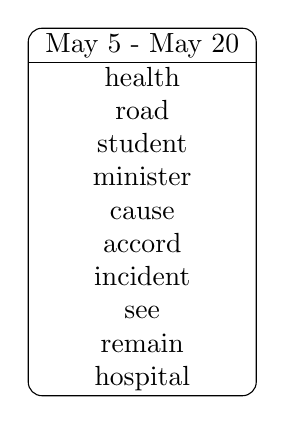
\begin{tikzpicture}
\node (table) [inner sep=0pt] {
\begin{tabular}{c}
{May 5 - May 20} \\
  \hline
health  \\
	road   \\
	student  \\
	minister  \\
	cause  \\
	accord   \\
	incident  \\
	see   \\
	remain  \\
	hospital \\
\end{tabular}
};
\draw [rounded corners=.5em] (table.north west) rectangle (table.south east);
\end{tikzpicture}
\label{dat_2_health_evoluation}
\end{table}

\begin{table}
\caption{Topic Distribution Evolution for Topic UK.(2 weeks as a time unit)}
\centering
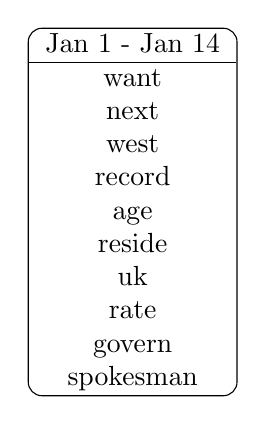
\begin{tikzpicture}
\node (table) [inner sep=0pt] {
\begin{tabular}{c}
  {Jan 1 - Jan 14} \\
  \hline
  want  \\
	next  \\
	west  \\
	record  \\
	age   \\
	reside  \\
	uk   \\
	rate  \\
	govern  \\
	spokesman   \\

\end{tabular}  
};
\draw [rounded corners=.5em] (table.north west) rectangle (table.south east);
\end{tikzpicture}
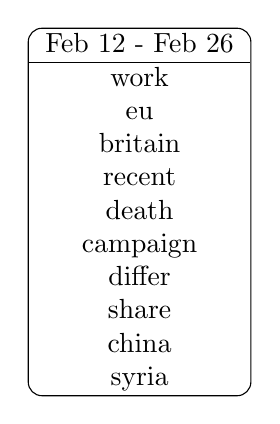
\begin{tikzpicture}
\node (table) [inner sep=0pt] {
\begin{tabular}{c}
{Feb 12 - Feb 26} \\
  \hline
 work  \\
	eu  \\
	britain  \\
	recent  \\
	death  \\
	campaign  \\
	differ  \\
	share  \\
	china \\
	syria  \\
\end{tabular}
};
\draw [rounded corners=.5em] (table.north west) rectangle (table.south east);
\end{tikzpicture}
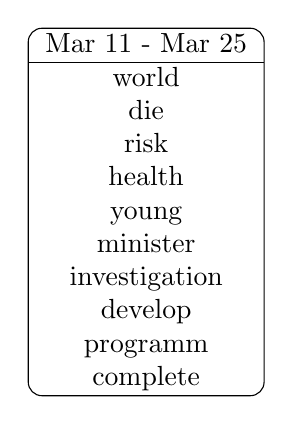
\begin{tikzpicture}
\node (table) [inner sep=0pt] {
\begin{tabular}{c}
{Mar 11 - Mar 25} \\
  \hline
 world   \\
	die   \\
	risk  \\
	health   \\
	young   \\
	minister  \\
	investigation   \\
	develop   \\
	programm   \\
	complete   \\
	
\end{tabular}
};
\draw [rounded corners=.5em] (table.north west) rectangle (table.south east);
\end{tikzpicture}
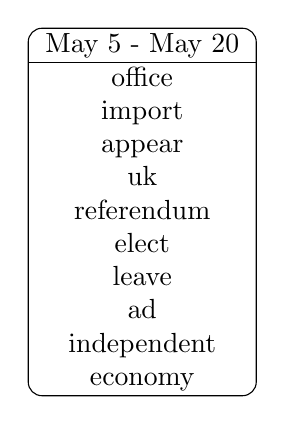
\begin{tikzpicture}
\node (table) [inner sep=0pt] {
\begin{tabular}{c}
{May 5 - May 20} \\
  \hline
office   \\
	import  \\
	appear \\
	uk  \\
	referendum   \\
	elect  \\
	leave   \\
	ad   \\
	independent   \\
	economy \\
\end{tabular}
};
\draw [rounded corners=.5em] (table.north west) rectangle (table.south east);
\end{tikzpicture}
\label{dat_2_uk_evoluation}
\end{table}

\begin{table}
\caption{Topic Distribution Evolution for Topic Educatoin.(2 weeks as a time unit)}
\centering
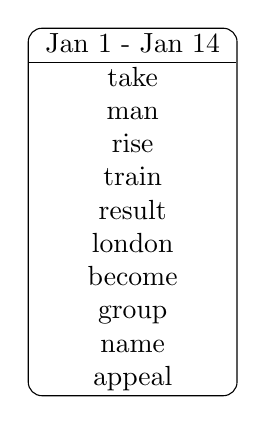
\begin{tikzpicture}
\node (table) [inner sep=0pt] {
\begin{tabular}{c}
  {Jan 1 - Jan 14} \\
  \hline
  take   \\
	man   \\
	rise  \\
	train  \\
	result \\
	london   \\
	become  \\
	group  \\
	name   \\
	appeal  \\

\end{tabular}  
};
\draw [rounded corners=.5em] (table.north west) rectangle (table.south east);
\end{tikzpicture}
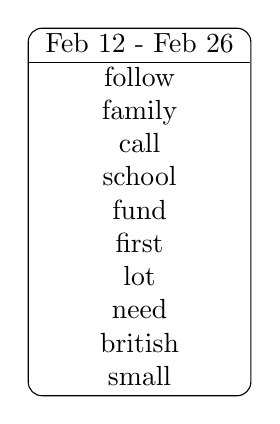
\begin{tikzpicture}
\node (table) [inner sep=0pt] {
\begin{tabular}{c}
{Feb 12 - Feb 26} \\
  \hline
 follow   \\
	family  \\
	call   \\
	school  \\
	fund   \\
	first   \\
	lot   \\
	need  \\
	british  \\
	small  \\
\end{tabular}
};
\draw [rounded corners=.5em] (table.north west) rectangle (table.south east);
\end{tikzpicture}
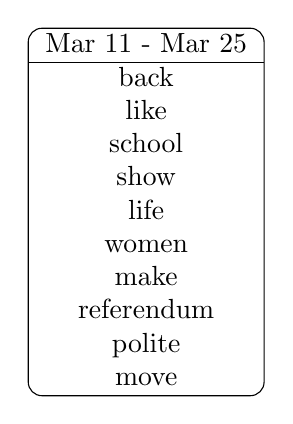
\begin{tikzpicture}
\node (table) [inner sep=0pt] {
\begin{tabular}{c}
{Mar 11 - Mar 25} \\
  \hline
 back  \\
	like   \\
	school \\
	show  \\
	life \\
	women  \\
	make  \\
	referendum  \\
	polite  \\
	move  \\

\end{tabular}
};
\draw [rounded corners=.5em] (table.north west) rectangle (table.south east);
\end{tikzpicture}
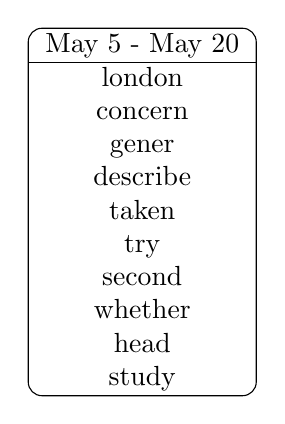
\begin{tikzpicture}
\node (table) [inner sep=0pt] {
\begin{tabular}{c}
{May 5 - May 20} \\
  \hline
london   \\
	concern   \\
	gener  \\
	describe \\
	taken\\
	try  \\
	second   \\
	whether \\
	head   \\
	study   \\
\end{tabular}
};
\draw [rounded corners=.5em] (table.north west) rectangle (table.south east);
\end{tikzpicture}
\label{dat_2_educatoin_evoluation}
\end{table}

\begin{table}
\caption{Topic Distribution Evolution for Topic Health.(4 weeks as a time unit)}
\centering
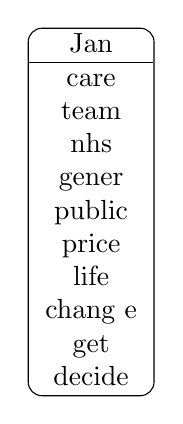
\begin{tikzpicture}
\node (table) [inner sep=0pt] {
\begin{tabular}{c}
  {Jan} \\
  \hline
  care  \\
	team  \\
	nhs   \\
	gener  \\
	public  \\
	price   \\
	life   \\
chang e  \\
	get \\
	decide \\
\end{tabular}  
};
\draw [rounded corners=.5em] (table.north west) rectangle (table.south east);
\end{tikzpicture}
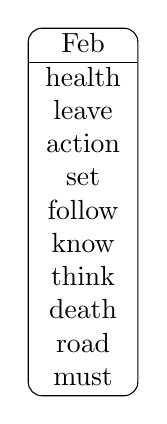
\begin{tikzpicture}
\node (table) [inner sep=0pt] {
\begin{tabular}{c}
{Feb} \\
  \hline
 health  \\
	leave  \\
	action  \\
	set   \\
	follow  \\
	know  \\
	think \\
	death  \\
	road  \\
	must  \\
\end{tabular}
};
\draw [rounded corners=.5em] (table.north west) rectangle (table.south east);
\end{tikzpicture}
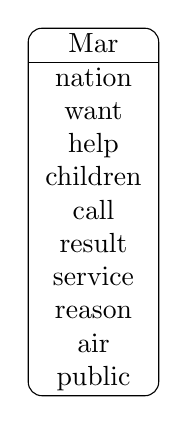
\begin{tikzpicture}
\node (table) [inner sep=0pt] {
\begin{tabular}{c}
{Mar} \\
  \hline
 nation   \\
	want  \\
	help  \\
	children  \\
	call   \\
	result   \\
	service   \\
	reason   \\
	air   \\
	public   \\
	
\end{tabular}
};
\draw [rounded corners=.5em] (table.north west) rectangle (table.south east);
\end{tikzpicture}
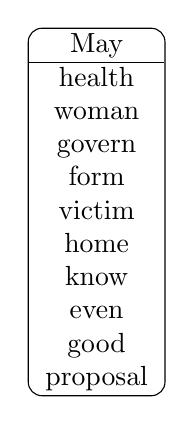
\begin{tikzpicture}
\node (table) [inner sep=0pt] {
\begin{tabular}{c}
{May} \\
  \hline
	health   \\
	woman   \\
	govern   \\
	form   \\
	victim   \\
	home  \\
	know  \\
	even   \\
	good   \\
	proposal  \\
	
\end{tabular}
};
\draw [rounded corners=.5em] (table.north west) rectangle (table.south east);
\end{tikzpicture}
\label{dat_4_health_evoluation}
\end{table}

\begin{table}
\caption{Topic Distribution Evolution for Topic UK.(4 weeks as a time unit)}
\centering
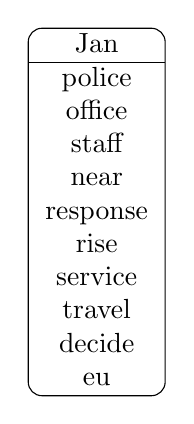
\begin{tikzpicture}
\node (table) [inner sep=0pt] {
\begin{tabular}{c}
  {Jan} \\
  \hline
  police  \\
	office   \\
	staff  \\
	near  \\
	response \\
	rise  \\
	service   \\
	travel   \\
	decide   \\
	eu\\

\end{tabular}  
};
\draw [rounded corners=.5em] (table.north west) rectangle (table.south east);
\end{tikzpicture}
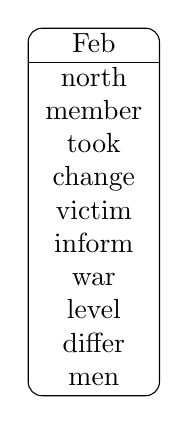
\begin{tikzpicture}
\node (table) [inner sep=0pt] {
\begin{tabular}{c}
{Feb} \\
  \hline
north   \\
	member   \\
	took   \\
	change  \\
	victim  \\
	inform  \\
	war   \\
	level  \\
	differ  \\
	men \\
\end{tabular}
};
\draw [rounded corners=.5em] (table.north west) rectangle (table.south east);
\end{tikzpicture}
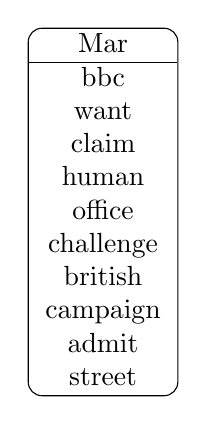
\begin{tikzpicture}
\node (table) [inner sep=0pt] {
\begin{tabular}{c}
{Mar} \\
  \hline
 bbc   \\
	want \\
	claim  \\
	human   \\
	office  \\
	challenge \\
	british  \\
	campaign  \\
	admit   \\
	street  \\
	
\end{tabular}
};
\draw [rounded corners=.5em] (table.north west) rectangle (table.south east);
\end{tikzpicture}
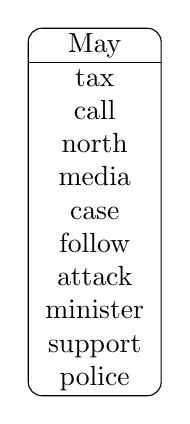
\begin{tikzpicture}
\node (table) [inner sep=0pt] {
\begin{tabular}{c}
{May} \\
  \hline
tax \\
	call   \\
	north   \\
	media  \\
	case  \\
	follow  \\
	attack  \\
	minister  \\
	support \\
	police  \\
\end{tabular}
};
\draw [rounded corners=.5em] (table.north west) rectangle (table.south east);
\end{tikzpicture}
\label{dat_2_uk_evoluation}
\end{table}

\begin{table}
\caption{Topic Distribution Evolution for Topic Educatoin.(4 weeks as a time unit)}
\centering
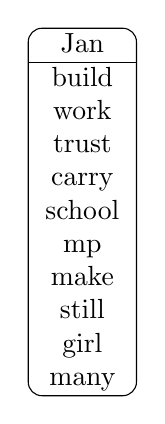
\begin{tikzpicture}
\node (table) [inner sep=0pt] {
\begin{tabular}{c}
  {Jan} \\
  \hline
 build  \\
	work  \\
	trust  \\
	carry  \\
	school   \\
	mp  \\
	make  \\
	still  \\
	girl  \\
	many  \\

\end{tabular}  
};
\draw [rounded corners=.5em] (table.north west) rectangle (table.south east);
\end{tikzpicture}
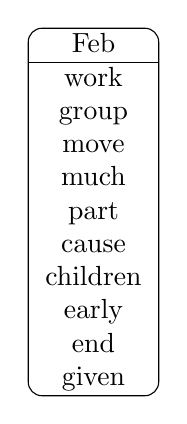
\begin{tikzpicture}
\node (table) [inner sep=0pt] {
\begin{tabular}{c}
{Feb} \\
  \hline
work  \\
	group   \\
	move  \\
	much \\
	part  \\
	cause  \\

	children  \\
	early  \\
	end  \\
	given  \\
\end{tabular}
};
\draw [rounded corners=.5em] (table.north west) rectangle (table.south east);
\end{tikzpicture}
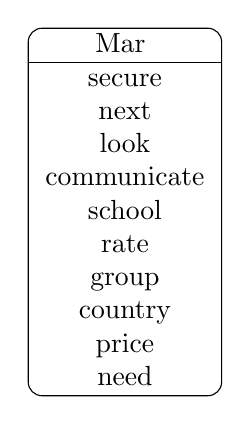
\begin{tikzpicture}
\node (table) [inner sep=0pt] {
\begin{tabular}{c}
{Mar } \\
  \hline
secure  \\
	next  \\
	look   \\
	communicate  \\
	school   \\
	rate   \\
	group   \\
	country  \\
	price   \\
	need  \\


\end{tabular}
};
\draw [rounded corners=.5em] (table.north west) rectangle (table.south east);
\end{tikzpicture}
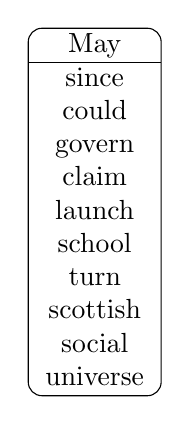
\begin{tikzpicture}
\node (table) [inner sep=0pt] {
\begin{tabular}{c}
{May} \\
  \hline
since  \\
	could   \\
	govern  \\
	claim   \\
	launch   \\
	school   \\
	turn   \\
	scottish   \\
	social   \\
	universe  \\
	\end{tabular}
};
\draw [rounded corners=.5em] (table.north west) rectangle (table.south east);
\end{tikzpicture}
\label{dat_2_educatoin_evoluation}
\end{table}